% Options for packages loaded elsewhere
\PassOptionsToPackage{unicode}{hyperref}
\PassOptionsToPackage{hyphens}{url}
%
\documentclass[
  12pt,
]{book}
\usepackage{amsmath,amssymb}
\usepackage{iftex}
\ifPDFTeX
  \usepackage[T1]{fontenc}
  \usepackage[utf8]{inputenc}
  \usepackage{textcomp} % provide euro and other symbols
\else % if luatex or xetex
  \usepackage{unicode-math} % this also loads fontspec
  \defaultfontfeatures{Scale=MatchLowercase}
  \defaultfontfeatures[\rmfamily]{Ligatures=TeX,Scale=1}
\fi
\usepackage{lmodern}
\ifPDFTeX\else
  % xetex/luatex font selection
\fi
% Use upquote if available, for straight quotes in verbatim environments
\IfFileExists{upquote.sty}{\usepackage{upquote}}{}
\IfFileExists{microtype.sty}{% use microtype if available
  \usepackage[]{microtype}
  \UseMicrotypeSet[protrusion]{basicmath} % disable protrusion for tt fonts
}{}
\makeatletter
\@ifundefined{KOMAClassName}{% if non-KOMA class
  \IfFileExists{parskip.sty}{%
    \usepackage{parskip}
  }{% else
    \setlength{\parindent}{0pt}
    \setlength{\parskip}{6pt plus 2pt minus 1pt}}
}{% if KOMA class
  \KOMAoptions{parskip=half}}
\makeatother
\usepackage{xcolor}
\usepackage[left=2.5cm,right=2.5cm,top=2cm,bottom=2cm]{geometry}
\usepackage{color}
\usepackage{fancyvrb}
\newcommand{\VerbBar}{|}
\newcommand{\VERB}{\Verb[commandchars=\\\{\}]}
\DefineVerbatimEnvironment{Highlighting}{Verbatim}{commandchars=\\\{\}}
% Add ',fontsize=\small' for more characters per line
\usepackage{framed}
\definecolor{shadecolor}{RGB}{248,248,248}
\newenvironment{Shaded}{\begin{snugshade}}{\end{snugshade}}
\newcommand{\AlertTok}[1]{\textcolor[rgb]{0.94,0.16,0.16}{#1}}
\newcommand{\AnnotationTok}[1]{\textcolor[rgb]{0.56,0.35,0.01}{\textbf{\textit{#1}}}}
\newcommand{\AttributeTok}[1]{\textcolor[rgb]{0.13,0.29,0.53}{#1}}
\newcommand{\BaseNTok}[1]{\textcolor[rgb]{0.00,0.00,0.81}{#1}}
\newcommand{\BuiltInTok}[1]{#1}
\newcommand{\CharTok}[1]{\textcolor[rgb]{0.31,0.60,0.02}{#1}}
\newcommand{\CommentTok}[1]{\textcolor[rgb]{0.56,0.35,0.01}{\textit{#1}}}
\newcommand{\CommentVarTok}[1]{\textcolor[rgb]{0.56,0.35,0.01}{\textbf{\textit{#1}}}}
\newcommand{\ConstantTok}[1]{\textcolor[rgb]{0.56,0.35,0.01}{#1}}
\newcommand{\ControlFlowTok}[1]{\textcolor[rgb]{0.13,0.29,0.53}{\textbf{#1}}}
\newcommand{\DataTypeTok}[1]{\textcolor[rgb]{0.13,0.29,0.53}{#1}}
\newcommand{\DecValTok}[1]{\textcolor[rgb]{0.00,0.00,0.81}{#1}}
\newcommand{\DocumentationTok}[1]{\textcolor[rgb]{0.56,0.35,0.01}{\textbf{\textit{#1}}}}
\newcommand{\ErrorTok}[1]{\textcolor[rgb]{0.64,0.00,0.00}{\textbf{#1}}}
\newcommand{\ExtensionTok}[1]{#1}
\newcommand{\FloatTok}[1]{\textcolor[rgb]{0.00,0.00,0.81}{#1}}
\newcommand{\FunctionTok}[1]{\textcolor[rgb]{0.13,0.29,0.53}{\textbf{#1}}}
\newcommand{\ImportTok}[1]{#1}
\newcommand{\InformationTok}[1]{\textcolor[rgb]{0.56,0.35,0.01}{\textbf{\textit{#1}}}}
\newcommand{\KeywordTok}[1]{\textcolor[rgb]{0.13,0.29,0.53}{\textbf{#1}}}
\newcommand{\NormalTok}[1]{#1}
\newcommand{\OperatorTok}[1]{\textcolor[rgb]{0.81,0.36,0.00}{\textbf{#1}}}
\newcommand{\OtherTok}[1]{\textcolor[rgb]{0.56,0.35,0.01}{#1}}
\newcommand{\PreprocessorTok}[1]{\textcolor[rgb]{0.56,0.35,0.01}{\textit{#1}}}
\newcommand{\RegionMarkerTok}[1]{#1}
\newcommand{\SpecialCharTok}[1]{\textcolor[rgb]{0.81,0.36,0.00}{\textbf{#1}}}
\newcommand{\SpecialStringTok}[1]{\textcolor[rgb]{0.31,0.60,0.02}{#1}}
\newcommand{\StringTok}[1]{\textcolor[rgb]{0.31,0.60,0.02}{#1}}
\newcommand{\VariableTok}[1]{\textcolor[rgb]{0.00,0.00,0.00}{#1}}
\newcommand{\VerbatimStringTok}[1]{\textcolor[rgb]{0.31,0.60,0.02}{#1}}
\newcommand{\WarningTok}[1]{\textcolor[rgb]{0.56,0.35,0.01}{\textbf{\textit{#1}}}}
\usepackage{longtable,booktabs,array}
\usepackage{calc} % for calculating minipage widths
% Correct order of tables after \paragraph or \subparagraph
\usepackage{etoolbox}
\makeatletter
\patchcmd\longtable{\par}{\if@noskipsec\mbox{}\fi\par}{}{}
\makeatother
% Allow footnotes in longtable head/foot
\IfFileExists{footnotehyper.sty}{\usepackage{footnotehyper}}{\usepackage{footnote}}
\makesavenoteenv{longtable}
\usepackage{graphicx}
\makeatletter
\def\maxwidth{\ifdim\Gin@nat@width>\linewidth\linewidth\else\Gin@nat@width\fi}
\def\maxheight{\ifdim\Gin@nat@height>\textheight\textheight\else\Gin@nat@height\fi}
\makeatother
% Scale images if necessary, so that they will not overflow the page
% margins by default, and it is still possible to overwrite the defaults
% using explicit options in \includegraphics[width, height, ...]{}
\setkeys{Gin}{width=\maxwidth,height=\maxheight,keepaspectratio}
% Set default figure placement to htbp
\makeatletter
\def\fps@figure{htbp}
\makeatother
\setlength{\emergencystretch}{3em} % prevent overfull lines
\providecommand{\tightlist}{%
  \setlength{\itemsep}{0pt}\setlength{\parskip}{0pt}}
\setcounter{secnumdepth}{5}
\usepackage{booktabs}
\usepackage{xcolor}
% \usepackage{amsmath}
\usepackage{bm}
\usepackage{geometry}
\usepackage{centernot}

\newcommand{\pr}[2][]{P_{#1}\left(#2\right)}
\newcommand{\spac}[1]{\mathcal{#1}}
\def \given {|}
\newcommand{\knowledge}{K}
\newcommand{\know}{\knowledge}
\newcommand{\e}[1]{{\textrm E}[#1]}
\newcommand{\var}[1]{{\textrm{Var}}[#1]}
\newcommand{\cov}[2]{{\textrm{Cov}}[#1,#2]}
\newcommand{\real}{{\mathbb R}}
\newcommand{\set}[1]{\{#1\}}
\newcommand{\st}{:\,}
\newcommand{\normal}{{\mathcal N}}
\newcommand{\natnos}{\mathbb{N}}
\newcommand{\logpr}[1]{l\left(#1\right)}
\newcommand{\hbeta}{\hat{\beta}}
\newcommand{\htheta}{\hat\theta}
\newcommand{\heta}{\hat\eta}
\newcommand{\hmu}{\hat\mu}
\newcommand{\hpi}{\hat\pi}
\newcommand{\hphi}{\hat\phi}
\newcommand{\isp}{\;}
\newcommand{\mc}{\mathcal}
\newcommand{\mb}[1]{\boldsymbol{#1}}
\newcommand{\eqa}{\stackrel{a}{=}}
\newcommand{\sat}[1]{#1_{\text{sat}}}
\newcommand{\sati}[1]{#1_{\text{sat},i}}
\newcommand{\tbeta}{\tilde\beta}
\ifLuaTeX
  \usepackage{selnolig}  % disable illegal ligatures
\fi
\usepackage[]{natbib}
\bibliographystyle{plainnat}
\usepackage{bookmark}
\IfFileExists{xurl.sty}{\usepackage{xurl}}{} % add URL line breaks if available
\urlstyle{same}
\hypersetup{
  pdftitle={Advanced Statistical Modelling III (Epiphany term)},
  pdfauthor={Department of Mathematical Sciences at Durham University},
  hidelinks,
  pdfcreator={LaTeX via pandoc}}

\title{Advanced Statistical Modelling III (Epiphany term)}
\author{Department of Mathematical Sciences at Durham University}
\date{09 Jan, 2025}

\begin{document}
\maketitle

{
\setcounter{tocdepth}{1}
\tableofcontents
}
\chapter*{General Information}\label{general-information}
\addcontentsline{toc}{chapter}{General Information}

\begin{itemize}
\tightlist
\item
  These are the lecture notes for the second term of the module MATH3411 -- Advanced Statistical Modelling III of Durham University's degree for Mathematics and Statistics.
\item
  \textbf{Acknowledgements}: This material is based on the lecture notes in previous modules taught by Dr Samuel Jackson, Dr Jochen Einbeck, Dr Ric Crossman, Dr Emmanuel Ogundimu, Dr Cuong Nguyen, Dr Ian Jermyn, Dr Louis Aslett, and Dr Reza Drikvandi.
\end{itemize}

\chapter{Introduction and Review}\label{introduction}

\renewcommand{\pr}[2][]{P_{#1}\left(#2\right)}
\renewcommand{\spac}[1]{\mathcal{#1}}
\renewcommand{\given}{|}
\renewcommand{\knowledge}{K}
\renewcommand{\know}{\knowledge}
\renewcommand{\e}[1]{{\mathrm E}[#1]}
\renewcommand{\var}[1]{{\mathrm{Var}}[#1]}
\renewcommand{\cov}[1]{{\mathrm{Cov}}[#1]}
\renewcommand{\real}{{\mathbb R}}
\renewcommand{\set}[1]{\left\{#1\right\}}
\renewcommand{\st}{:\,}
\renewcommand{\normal}{{\mathcal N}}
\renewcommand{\natnos}{\mathbb{N}}
\renewcommand{\isp}{\;}
\renewcommand{\mc}{\mathcal}
\renewcommand{\hbeta}{\hat{\mb{\beta}}}
\renewcommand{\mb}[1]{\boldsymbol{#1}}
\renewcommand{\eqa}{\stackrel{a}{=}}
\renewcommand{\logpr}[1]{l\left(#1\right)}

\section{Introduction}\label{introduction-1}

In the first term, we have learned about categorical data analysis and some basics of generalised linear models (GLMs). In this term, we will continue to explore GLMs in more detail and study some of its more general variants. In particular, we will learn:

\begin{itemize}
\item
  How to estimate the parameters of a GLM from data.
\item
  How to make a prediction and do inference once a GLM has been fitted.
\item
  How to perform deviance analysis with GLMs.
\item
  How to reduce overdispersion using quasi-likelihood methods.
\item
  How to model repeated measures data using marginal models.
\item
  How to model mixed effects using linear mixed models (LMMs) and generalised linear mixed models (GLMMs).
\end{itemize}

For the rest of this chapter, we will review some random vector and random matrix identities that will be useful later. Then we will review the basics of GLMs.

\section{Random Vectors and Random Matrices: A Review}\label{ranmat}

\begin{itemize}
\tightlist
\item
  A \emph{random vector} is a vector of random variables:
\end{itemize}

\[\boldsymbol{X} = \left(\begin{array}{c} X_1 \\ \vdots \\ X_n \end{array}\right).\]

\begin{itemize}
\tightlist
\item
  The mean or expectation of \(\boldsymbol{X}\) is defined as:
\end{itemize}

\[E[\boldsymbol{X}] = \left(\begin{array}{c} E[X_1] \\ \vdots \\ E[X_n] \end{array}\right).\]

\begin{itemize}
\tightlist
\item
  A \emph{random matrix} is a matrix of random variables:
\end{itemize}

\[
\boldsymbol{Z} = (Z_{ij}) =
\left(\begin{array}{ccc} Z_{11} & \ldots & Z_{1m} \\
                         \vdots & \ddots & \vdots \\
                         Z_{n1} & \ldots & Z_{nm} \end{array}\right).
\]

\begin{itemize}
\tightlist
\item
  The expectation of \(\boldsymbol{Z}\) is defined as:
\end{itemize}

\[
E[\boldsymbol{Z}] = (E[Z_{ij}]) =
\left(\begin{array}{ccc} E[Z_{11}] & \ldots & E[Z_{1m}] \\
                         \vdots    & \ddots & \vdots    \\
                         E[Z_{n1}] & \ldots & E[Z_{nm}] \end{array}\right).
\]

\begin{itemize}
\item
  Some properties of random vectors and random matrices:

  \begin{itemize}
  \item
    If \(\boldsymbol{a}\) is a constant (i.e., non-random) vector, \(E[\boldsymbol{a}] = \boldsymbol{a}\).
  \item
    If \(\boldsymbol{A}\) is a constant matrix, \(E[\boldsymbol{A}] = \boldsymbol{A}\).
  \item
    \(E[\boldsymbol{X} + \boldsymbol{Y}] = E[\boldsymbol{X}] + E[\boldsymbol{Y}]\) for any random matrices \(\boldsymbol{X}\) and \(\boldsymbol{Y}\).
  \item
    \(E[\boldsymbol{A}\boldsymbol{X}] = \boldsymbol{A} E[\boldsymbol{X}]\) for a constant matrix \(\boldsymbol{A}\) and a random matrix \(\boldsymbol{X}\).
  \item
    More generally, \(E[\boldsymbol{A}\boldsymbol{X}\boldsymbol{B} + \boldsymbol{C}] = \boldsymbol{A}E[\boldsymbol{X}]\boldsymbol{B} + \boldsymbol{C}\) for constant matrices \(\boldsymbol{A}\), \(\boldsymbol{B}\) and \(\boldsymbol{C}\).
  \end{itemize}
\item
  Let \(\boldsymbol{X}\) be a random vector. The \emph{covariance matrix} of \(\boldsymbol{X}\) is defined as:
\end{itemize}

\[
cov(\boldsymbol{X}) = (cov(X_i, X_j)) =
\left(\begin{array}{cccc} var(X_1)      & cov(X_1, X_2) & \ldots & cov(X_1, X_n) \\
                          cov(X_2, X_1) & var(X_2)      & \ldots & cov(X_2, X_n) \\
                          \vdots        & \vdots        & \ddots & \vdots        \\
                          cov(X_n, X_1) & cov(X_n, X_2) & \ldots & var(X_n) \end{array}\right).
\]

\begin{itemize}
\tightlist
\item
  We can also write:
\end{itemize}

\[\begin{aligned}
cov(\boldsymbol{X}) &= E[(\boldsymbol{X} - E[\boldsymbol{X}])(\boldsymbol{X} - E[\boldsymbol{X}])^T] \\
&= E\left[ \left(\begin{array}{c} X_1 - E[X_1] \\ \vdots \\ X_n - E[X_n] \end{array}\right) \left( X_1 - E[X_1], \ldots, X_n - E[X_n] \right) \right].
\end{aligned}\]

\begin{itemize}
\item
  Some properties of covariance matrices:

  \begin{itemize}
  \item
    They are symmetric: \(cov(\boldsymbol{X}) = cov(\boldsymbol{X})^T\).
  \item
    If \(\boldsymbol{a}\) is a constant vector, \(cov(\boldsymbol{X} + \boldsymbol{a}) = cov(\boldsymbol{X})\).
  \item
    If \(\boldsymbol{A}\) is a constant matrix, \(cov(\boldsymbol{A} \boldsymbol{X}) = \boldsymbol{A} cov(\boldsymbol{X}) \boldsymbol{A}^T\).
  \item
    \(cov(\boldsymbol{X}) = E[\boldsymbol{X} \boldsymbol{X}^T] - E[\boldsymbol{X}]  E[\boldsymbol{X}]^T\).
  \end{itemize}
\item
  Let \(\boldsymbol{X}_{n \times 1}\) and \(\boldsymbol{Y}_{m \times 1}\) be random vectors where \(n\) and \(m\) could be different. The covariance matrix of \(\boldsymbol{X}\) and \(\boldsymbol{Y}\) is defined as:
\end{itemize}

\[
cov(\boldsymbol{X}, \boldsymbol{Y}) = (cov(X_i, Y_j)) =
\left(\begin{array}{cccc} cov(X_1, Y_1) & cov(X_1, Y_2) & \ldots & cov(X_1, Y_m) \\
                          cov(X_2, Y_1) & cov(X_2, Y_2) & \ldots & cov(X_2, Y_m) \\
                          \vdots        & \vdots        & \ddots & \vdots        \\
                          cov(X_n, Y_1) & cov(X_n, Y_2) & \ldots & cov(X_n, Y_m) \end{array}\right).
\]

\begin{itemize}
\tightlist
\item
  We can also write:
\end{itemize}

\[\begin{aligned}
cov(\boldsymbol{X}, \boldsymbol{Y}) &= E[(\boldsymbol{X} - E[\boldsymbol{X}])(\boldsymbol{Y} - E[\boldsymbol{Y}])^T] \\
&= E\left[ \left(\begin{array}{c} X_1 - E[X_1] \\ \vdots \\ X_n - E[X_n] \end{array}\right) \left( Y_1 - E[Y_1], \ldots, Y_m - E[Y_m] \right) \right].
\end{aligned}\]

\begin{itemize}
\item
  Some properties of covariance matrices between two vectors:

  \begin{itemize}
  \item
    If \(\boldsymbol{A}\) and \(\boldsymbol{B}\) are constant matrices, \(cov(\boldsymbol{A} \boldsymbol{X}, \boldsymbol{B} \boldsymbol{Y}) = \boldsymbol{A} cov(\boldsymbol{X},  \boldsymbol{Y}) \boldsymbol{B}^T.\)
  \item
    If \(\boldsymbol{Z} = \left(\begin{array}{c} \boldsymbol{X} \\ \boldsymbol{Y} \end{array}\right)\), then \(cov(\boldsymbol{Z}) = \left(\begin{array}{cc} cov(\boldsymbol{X}) & cov(\boldsymbol{X}, \boldsymbol{Y}) \\ cov(\boldsymbol{Y}, \boldsymbol{X}) & cov(\boldsymbol{Y}) \end{array}\right)\).
  \end{itemize}
\item
  Let \(\boldsymbol{X}\) be a random vector. The \emph{correlation matrix} of \(\boldsymbol{X}\) is defined as:
\end{itemize}

\[
corr(\boldsymbol{X}) = (corr(X_i, X_j)) =
\left(\begin{array}{cccc} 1              & corr(X_1, X_2) & \ldots & corr(X_1, X_n) \\
                          corr(X_2, X_1) & 1              & \ldots & corr(X_2, X_n) \\
                          \vdots         & \vdots         & \ddots & \vdots         \\
                          corr(X_n, X_1) & corr(X_n, X_2) & \ldots & 1 \end{array}\right),
\]
where

\[corr(X_i, X_j) = \frac{cov(X_i, X_j)}{\sqrt{var(X_i) var(X_j)}}.\]

\section{Generalised Linear Models: A Review}\label{generalised-linear-models-a-review}

Generalised linear models (GLMs) are developed by \citet{nelder1972generalized} as a way to unify other statistical models as well as the statistical methods operated on these models. In this section, we will briefly review the definition of GLMs. Please refer to the last term's lecture notes for more detailed derivations and examples.

\textbf{Definition.} A GLM is specified through the following components:

\begin{itemize}
\item
  A \emph{linear predictor}: \(\eta = \boldsymbol{\beta}^{T}\boldsymbol{x}\).
\item
  An \emph{injective response function} \(h\), such that \(\mu = {\mathrm E}[Y |\boldsymbol{x}, \boldsymbol{\beta}] = h(\eta) = h(\boldsymbol{\beta}^{T}\boldsymbol{x})\).\\
  Equivalently, one can write \(g(\mu) = \boldsymbol{\beta}^{T}\boldsymbol{x}\), where \(g = h^{-1}\) is the \emph{link} function.
\item
  The \emph{distributional assumption}: \(P_{}\left(Y |\boldsymbol{x}, \boldsymbol{\beta}\right)\) is an EDF, that is:
  \begin{equation}
        P_{}\left(y |\boldsymbol{x}, \boldsymbol{\beta}\right)
        =
        P_{}\left(y |\theta(\boldsymbol{x}, \boldsymbol{\beta}), \phi(\boldsymbol{x}, \boldsymbol{\beta})\right)
        = \exp
        \Big(
            \frac{y\theta - b(\theta)}{\phi} + c(y, \phi)
        \Big).
    \end{equation}
  From the properties of the EDF, the mean and variance of this distribution are:
  \begin{align}
    {\mathrm E}[Y |\theta, \phi] &= \mu = b'(\theta) 
    \\
    {\mathrm{Var}}[Y |\theta, \phi] &= \phi \, b''(\theta) = \phi \, b''((b')^{-1}(\mu)) = \phi \, \mathcal{V}(\mu).
  \end{align}
\item
  We also assume \emph{independent data}, that is:
  \begin{equation}
        P_{}\left(\left\{y_{i}\right\} |\left\{\boldsymbol{x}_{i}\right\}, \boldsymbol{\beta}\right)
        =
        \prod_{i=1}^n
        P_{}\left(y_{i} |\boldsymbol{x}_{i}, \boldsymbol{\beta}\right)
    \end{equation}
  where \(\left\{y_{i}, i = 1,...,n\right\}\) are response data given the \(\left\{\boldsymbol{x}_i, i = 1,...,n\right\}\).
\end{itemize}

\textbf{The Natural/Canonical Link.} Recall that we have both:
\begin{alignat}{4}
\mu & =  {\mathrm E}[Y |\theta, \phi] && =  b'(\theta) 
\label{eq:meanbtheta}
\\
\mu & =  {\mathrm E}[Y |\boldsymbol{x}, \boldsymbol{\beta}] && =  h(\boldsymbol{\beta}^T\boldsymbol{x})  =  h(\eta)
\label{eq:meanh}
\end{alignat}
with Equation \eqref{eq:meanbtheta} holding as a result of
\(P_{}\left(y |\theta, \phi\right)\)
following an EDF distribution, and Equation \eqref{eq:meanh} holding by definition for a GLM.

The \emph{natural link} is the choice \(h = b'\), or equivalently \(g = (b')^{-1}\), resulting in the equation
\begin{equation}
 \theta = \boldsymbol{\beta}^T\boldsymbol{x} = \eta.
\end{equation}

\section{Exercises}\label{exercises}

\begin{enumerate}
\def\labelenumi{\arabic{enumi}.}
\item
  Prove the identities in Section \ref{ranmat}.
\item
  The table below gives some common link functions for GLMs. In the table, \(\Phi(\cdot)\) is the cdf of the standard normal distribution. Find their inverses (i.e., the response function \(h\)).
\end{enumerate}

\begin{longtable}[]{@{}ll@{}}
\toprule\noalign{}
Link function & \(\eta_i = g(\mu_i)\) \\
\midrule\noalign{}
\endhead
\bottomrule\noalign{}
\endlastfoot
Identity & \(\mu_i\) \\
Log & \(\log(\mu_i)\) \\
Inverse & \(\mu_i^{-1}\) \\
Inverse-square & \(\mu_i^{-2}\) \\
Square-root & \(\sqrt{\mu_i}\) \\
Logit & \(\log\frac{\mu_i}{1-\mu_i}\) \\
Probit & \(\Phi^{-1}(\mu_i)\) \\
Log-log & \(-\log(-\log\mu_i)\) \\
Complementary log-log & \(\log(-\log(1-\mu_i))\) \\
\end{longtable}

\begin{enumerate}
\def\labelenumi{\arabic{enumi}.}
\setcounter{enumi}{2}
\tightlist
\item
  Write down the GLM components and the corresponding natural link when the response variable \(Y\) is assumed to follow each distribution below. Note that the values of \(y_i\) have to be in the correct range for each distribution.
\end{enumerate}

\begin{itemize}
\item
  Gaussian: \(y_i |\boldsymbol{x}_i, \boldsymbol{\beta} \sim \mathcal{N}(\mu_i, \sigma^2)\).
\item
  Bernoulli: \(y_i |\boldsymbol{x}_i, \boldsymbol{\beta} \sim Bernoulli(\mu_i)\).
\item
  Binomial: \(y_i |\boldsymbol{x}_i, \boldsymbol{\beta} \sim Bin(n_i, \mu_i)\). Note that here \(y_i\) is the proportion of successes in \(n_i\) independent trials with probability of success \(\mu_i\). Thus, the range of \(y_i\) is \(\{ \frac{0}{n_i}, \frac{1}{n_i}, \ldots, \frac{n_i}{n_i} \}\).
\item
  Poisson: \(y_i |\boldsymbol{x}_i, \boldsymbol{\beta} \sim Poi(\mu_i)\).
\item
  Gamma: \(y_i |\boldsymbol{x}_i, \boldsymbol{\beta} \sim Gamma(\nu, \alpha_i)\), where \(\nu\) and \(\alpha_i\) are the shape and rate parameters of the Gamma distribution.
\item
  Inverse-Gaussian: \(y_i |\boldsymbol{x}_i, \boldsymbol{\beta} \sim IG(\mu_i, \lambda)\).
\end{itemize}

From these results, show that the linear regression model, logistic regression model, and Poisson regression model are all special cases of GLMs.

\begin{enumerate}
\def\labelenumi{\arabic{enumi}.}
\setcounter{enumi}{3}
\tightlist
\item
  In \(\texttt{R}\), find the default link function for each GLM family. Are they the natural link for the corresponding family?
\end{enumerate}

\chapter{Estimation}\label{estimation}

\renewcommand{\pr}[2][]{P_{#1}\left(#2\right)}
\renewcommand{\spac}[1]{\mathcal{#1}}
\renewcommand{\given}{|}
\renewcommand{\knowledge}{K}
\renewcommand{\know}{\knowledge}
\renewcommand{\e}[1]{{\mathrm E}[#1]}
\renewcommand{\var}[1]{{\mathrm{Var}}[#1]}
\renewcommand{\cov}[1]{{\mathrm{Cov}}[#1]}
\renewcommand{\real}{{\mathbb R}}
\renewcommand{\set}[1]{\left\{#1\right\}}
\renewcommand{\st}{:\,}
\renewcommand{\normal}{{\mathcal N}}
\renewcommand{\natnos}{\mathbb{N}}
\renewcommand{\isp}{\;}
\renewcommand{\mc}{\mathcal}
\renewcommand{\hbeta}{\hat{\mb{\beta}}}
\renewcommand{\mb}[1]{\boldsymbol{#1}}

Suppose we are given a dataset that we would like to model using a GLM. After checking the data and possibly performing some exploratory data analysis, we have already chosen a specific form of GLMs that is most suitable for the dataset (say e.g., the Poisson GLM). Now we wish to estimate the parameters of the model; that is, finding the value of \(\boldsymbol{\beta}\) that best explains our data. For this purpose, we can use the maximum likelihood method to obtain an estimate \(\hat{\boldsymbol{\beta}}\).

One advantage of the GLM formulation is that it allows us to derive a solution for the maximum likelihood method directly in the general form, thus unifying the estimation methods for various statistical models. In other words, we do not need to derive solutions for the Poisson GLM, the Binomial GLM, etc. separately. Instead, we can just derive the solution for the general form of the GLMs. The solution for each specific form of the GLM will be an instance of this general solution.

For the rest of this chapter,

\section{Likelihood Function}\label{likelihood-function}

Consider the grouped data setup where we have predictors and data with possible replicates \(\left\{(\boldsymbol{x}_{i}, y_{ir_{i}})\right\}_{i\in[1..n], r_{i}\in[1..m_{i}]}\).
Recall that under a GLM, given predictors \(\left\{\boldsymbol{x}_{i}\right\}_{i\in[1..n]}\), each response \(y_{ir_{i}}\) is independent of the other \(y_{jr_{j}}\), and of the values of all predictors \(\boldsymbol{x}_{j}\) with \(j\neq i\), so that the joint probability of the data --- that is, the likelihood --- is given by

\begin{equation}
  L(\boldsymbol{\beta}) 
  = P_{}\left(\left\{y_{ir_{i}}\right\} |\left\{\boldsymbol{x}_{i}\right\}, \boldsymbol{\beta}\right)
  = P_{}\left(\left\{y_{ir_{i}}\right\} |\left\{\theta_{i}\right\}, \phi\right)
  = \prod_{i = 1}^{n} \prod_{r_{i} = 1}^{m_{i}} P_{}\left(y_{ir_{i}} |\theta_{i}, \phi\right)
  \label{eq:jointprobability}
\end{equation}

where

\begin{equation}
  P_{}\left(y_{ir_{i}} |\theta_{i}, \phi\right)
  = \exp \left( \frac{y_{ir_{i}}\theta_{i} - b(\theta_{i})}{ \phi} + c(y_{ir_{i}}, \phi) \right)
\end{equation}

with

\begin{equation}
  \theta_{i}
  = (b')^{-1}(\mu_{i})
  = (b')^{-1}(h(\eta_{i}))
  = (b')^{-1}(h(\boldsymbol{\beta}^{T}\boldsymbol{x}_{i})).
\end{equation}

\section{Log-Likelihood Function}\label{loglike}

The log probability of the data --- or log-likelihood --- is thus given by

\begin{align}
  l(\boldsymbol{\beta})
  & = \log L(\boldsymbol{\beta}) = \log P_{}\left(\left\{y_{ir_{i}}\right\} |\left\{\theta_{i}\right\}, \phi\right) \\
  & = \sum_{i} \sum_{r_{i}} \left( \frac{y_{ir_{i}}\theta_{i} - b(\theta_{i})}{\phi} + c(y_{ir_{i}}, \phi) \right) \\
  & = \sum_{i} \left( m_{i} \frac{y_{i}\theta_{i} - b(\theta_{i})}{\phi} + \sum_{r_{i}} c(y_{ir_{i}}, \phi) \right) \\
  & = \sum_{i} l_{i}
\end{align}

where we have defined

\begin{align}
  y_i &= \frac{1}{m_i} \sum_{r_{i}} y_{ir_{i}} \\
  l_i &= \frac{y_{i}\theta_{i} - b(\theta_{i})}{\phi_i} + \sum_{r_{i}} c(y_{ir_{i}}, \phi) \\
  \phi_i &= \phi/m_i.
\end{align}

\section{Score Function and Score Equation}\label{score-function-and-score-equation}

The \emph{score function} is given by

\begin{equation}
  \boldsymbol{S}(\boldsymbol{\beta})
  = \frac{\partial l}{\partial \boldsymbol{\beta}^{T}}
  = \sum_{i} \frac{\partial l_{i}}{\partial \boldsymbol{\beta}^{T}}
  = \sum_{i} \frac{\partial l_{i}}{\partial \theta_{i}} 
             \frac{\partial \theta_{i}}{\partial \mu_{i}}
             \frac{\partial \mu_{i}}{\partial \eta_{i}}
             \frac{\partial \eta_{i}}{\partial \boldsymbol{\beta}^{T}}
  \label{eq:scorefunction}
\end{equation}

where, recalling that \(\mu_i = b'(\theta_i)\), \(\mathcal{V}(\mu_{i}) = b''(\theta_{i})\), \(\mu_i = h(\eta_i)\) and \(\eta_i = \boldsymbol{\beta}^T\boldsymbol{x}_i\), we have:\footnote{Note that here and in this module, we assume that \(\phi\) does not depend on \(\boldsymbol{\beta}\).}

\begin{align}
  \frac{\partial l_{i} }{\partial \theta_{i}}
    & = \frac{y_{i} - b'(\theta_{i})}{\phi_{i}}
      = \frac{y_{i} - \mu_{i}}{\phi_{i}} \\
  \frac{\partial \theta_{i}}{\partial \mu_{i}}
    & = 1 / \left( \frac{\partial \mu_{i}}{\partial \theta_{i}} \right)
      = \frac{1}{b''(\theta_{i})}
      = \frac{1}{\mathcal{V}(\mu_{i})}
      \label{eq:dthetadmu} \\
  \frac{\partial \mu_{i}}{\partial \eta_{i}}
    & = h'(\eta_{i})
      \label{eq:dmudeta} \\
  \frac{\partial \eta_{i}}{\partial \boldsymbol{\beta}^{T}}
    & = \boldsymbol{x}_{i}.
\end{align}

The score function is thus given by

\begin{align}
  \boldsymbol{S}(\boldsymbol{\beta})
  & = \sum_{i} \left(\frac{y_{i} - \mu_{i}}{\phi_{i}} \right) \;
               \left(\frac{1}{\mathcal{V}(\mu_{i})} \right) \;
               h'(\eta_{i}) \;\boldsymbol{x}_{i} \\
  & = \frac{1}{\phi} \sum_{i} m_{i}(y_{i} - \mu_{i}) \;
                              \frac{1}{\mathcal{V}(\mu_{i})} \;
                              h'(\eta_{i}) \;\boldsymbol{x}_{i}.
  \label{eq:scorefunction2}
\end{align}

The maximum likelihood estimate \(\hat{\boldsymbol{\beta}}\) must then satisfy the \emph{score equation}:

\begin{equation}
  \boldsymbol{S}(\hat{\boldsymbol{\beta}}) = 0.
  \label{eq:scoreequation}
\end{equation}

Note that the dispersion parameter \(\phi\) cancels from the score equation, which implies that \(\hat{\boldsymbol{\beta}}\) does not depend on \(\phi\). This is another important property of EDFs.

\subsection{Special Case: Natural Link}\label{special-case-natural-link}

For the natural link, \(\theta_{i} = \eta_{i}\), so Equations \eqref{eq:dthetadmu} and \eqref{eq:dmudeta} combine to give

\begin{equation}
  \frac{h'(\eta_i)}{\mathcal{V}(\mu_i)} 
  = \frac{\partial\theta_{i}}{\partial \mu_{i}} \frac{\partial\mu_{i}}{\partial \eta_{i}} 
  = \frac{\partial\theta_{i}}{\partial \eta_{i}} 
  = 1.
\end{equation}

The score function thus simplifies to

\begin{equation}
  \boldsymbol{S}(\boldsymbol{\beta}) = \frac{1}{\phi}\sum_{i} m_{i}(y_{i} - \mu_{i})\;\boldsymbol{x}_{i}.
  \label{eq:scorefunctionnaturallink}
\end{equation}

\section{Fisher Information}\label{fisherinformation}

To solve the score equation, we will also need the second derivative of the log-likelihood. Its negative is called the \emph{Observed Fisher Information}, defined as

\begin{equation}
  \boldsymbol{F}_{\text{obs}}(\boldsymbol{\beta})
  = - \frac{\partial^{2} l}{\partial\boldsymbol{\beta}^{T}\partial\boldsymbol{\beta}}
  = - \frac{\partial \boldsymbol{S}}{\partial \boldsymbol{\beta}}.
  \label{eq:observedfisherinformation}
\end{equation}

Note that, at the MLE, \(\boldsymbol{F}_{\text{obs}}(\hat{\boldsymbol{\beta}})\) is positive by definition.
Because it is a function of the data \(\left\{y_{i}\right\}\), \(\boldsymbol{F}_{\text{obs}}\) has a probability distribution. In practice, the Observed Fisher Information is often approximated by the \emph{Expected Fisher Information}, otherwise known simply as the \emph{Fisher Information}:\footnote{Some texts refer to \(\boldsymbol{F}_{\text{obs}}(\hat{\boldsymbol{\beta}})\) as the Observed Fisher Information, and to \(\boldsymbol{F}_{\text{obs}}(\boldsymbol{\beta})\) simply as the Fisher Information. Some don't refer to either of these at all. Just to be clear, we will refer to \(\boldsymbol{F}_{\text{obs}}(\boldsymbol{\beta})\) as the Observed Fisher Information and the Expected Fisher Information \(\boldsymbol{F}(\boldsymbol{\beta})\) simply as the Fisher Information.}

\begin{equation}
  \boldsymbol{F}(\boldsymbol{\beta}) = E \left[ - \frac{\partial \boldsymbol{S} }{ \partial \boldsymbol{\beta}} \right]
  \label{eq:fisherinformation}
\end{equation}

where the expectation is taken over the joint probability distribution of the data \(P_{}\left(\left\{y_{ir_{i}}\right\} |\boldsymbol{\beta}, \left\{\boldsymbol{x}_{i}\right\}\right)\).

\section{Example: Poisson Regression}\label{example-poisson-regression}

We look at two example calculations of the score function and Fisher Information for Poisson Regression, that is we have

\begin{itemize}
\tightlist
\item
  \(y |\boldsymbol{x}, \boldsymbol{\beta} \sim \text{Poi}(\lambda(\boldsymbol{x}, \boldsymbol{\beta}))\)
\item
  \(\phi = 1\).
\end{itemize}

In this example, let us assume \(m_i = 1\), i.e., the data are ungrouped.

\subsection{With Natural Link}\label{with-natural-link}

We have that:
\(\lambda(\boldsymbol{x}, \boldsymbol{\beta}) = \mu(\boldsymbol{x}, \boldsymbol{\beta}) = h(\eta(\boldsymbol{x}, \boldsymbol{\beta})) = e^{\eta(\boldsymbol{x}, \boldsymbol{\beta})} = e^{\boldsymbol{\beta}^T\boldsymbol{x}}\).

Equation \eqref{eq:scorefunctionnaturallink} then gives

\begin{equation}
  \boldsymbol{S}(\boldsymbol{\beta}) = \sum_{i} (y_{i} - e^{\boldsymbol{\beta}^{T}\boldsymbol{x}_{i}})\;\boldsymbol{x}_{i}
\end{equation}

while Equation \eqref{eq:observedfisherinformation} gives

\begin{equation}
  \boldsymbol{F}_{\text{obs}}(\boldsymbol{\beta}) = \sum_{i} e^{\boldsymbol{\beta}^{T}\boldsymbol{x}_{i}}\;\boldsymbol{x}_{i}\boldsymbol{x}_{i}^{T}.
\end{equation}

Note that this does not depend on the data, so that Equation \eqref{eq:fisherinformation} gives

\begin{equation}
  \boldsymbol{F}(\boldsymbol{\beta}) = {\mathrm E}[\boldsymbol{F}_{\text{obs}}(\boldsymbol{\beta})] = \boldsymbol{F}_{\text{obs}}(\boldsymbol{\beta}).
\end{equation}

\subsection{With Identity Link}\label{with-identity-link}

The identity link is defined such that \(h(\eta) = \eta\).

In this case, we have that:

\begin{itemize}
\tightlist
\item
  \(\lambda(\boldsymbol{x}, \boldsymbol{\beta}) = \mu(\boldsymbol{x}, \boldsymbol{\beta}) = h(\eta(\boldsymbol{x}, \boldsymbol{\beta})) = \eta(\boldsymbol{x}, \boldsymbol{\beta}) = \boldsymbol{\beta}^T \boldsymbol{x}\).
\item
  \(\mathcal{V}(\mu) = \mu\) (see Poisson example in EDF chapter).
\item
  \(h'(\eta) = 1\).
\end{itemize}

Equation \eqref{eq:scorefunction2} thus gives

\begin{align}
  \boldsymbol{S}(\boldsymbol{\beta})
  & = \sum_{i} (y_{i} - \mu_{i})\;\frac{1}{\mu_{i}}\;1 \;\boldsymbol{x}_{i} \\
  & = \sum_{i} (y_{i} - \boldsymbol{\beta}^{T}\boldsymbol{x}_{i}) \;\frac{1}{\boldsymbol{\beta}^{T}\boldsymbol{x}_{i}}\;\boldsymbol{x}_{i} \\
  & = \sum_{i} \left( \frac{y_{i}}{ \boldsymbol{\beta}^{T}\boldsymbol{x}_{i}} - 1 \right) \;\boldsymbol{x}_{i}.
\end{align}

Using Equation \eqref{eq:observedfisherinformation} and the chain rule, we can obtain the Observed Fisher Information:

\begin{equation}
  \boldsymbol{F}_{\text{obs}}(\boldsymbol{\beta})
  = \sum_{i} \frac{y_{i}}{ (\boldsymbol{\beta}^{T}\boldsymbol{x}_{i})^{2}}\;\boldsymbol{x}_{i}\boldsymbol{x}_{i}^{T}.
\end{equation}

Hence, the Fisher Information is:

\begin{align}
  \boldsymbol{F}(\boldsymbol{\beta})
  & = {\mathrm E}[\boldsymbol{F}_{\text{obs}}(\boldsymbol{\beta})] \\
  & = \textrm{E} \left[ \sum_{i} \frac{Y_{i}}{(\boldsymbol{\beta}^{T}\boldsymbol{x}_{i})^{2}} \;\boldsymbol{x}_{i}\boldsymbol{x}_{i}^{T} \right] \\
  & = \sum_{i} \frac{{\mathrm E}[Y_{i} |\boldsymbol{\beta}, \boldsymbol{x}_{i}]}{ (\boldsymbol{\beta}^{T}\boldsymbol{x}_{i})^{2}} \;\boldsymbol{x}_{i}\boldsymbol{x}_{i}^{T} \\
  & = \sum_{i} \frac{\boldsymbol{\beta}^{T}\boldsymbol{x}_{i} }{ (\boldsymbol{\beta}^{T}\boldsymbol{x}_{i})^{2}} \;\boldsymbol{x}_{i}\boldsymbol{x}_{i}^{T} \\
  & = \sum_{i} \frac{1 }{ \boldsymbol{\beta}^{T}\boldsymbol{x}_{i}}\;\boldsymbol{x}_{i}\boldsymbol{x}_{i}^{T}.
\end{align}

Note that \(\boldsymbol{F}(\boldsymbol{\beta}) \neq \boldsymbol{F}_{\text{obs}}(\boldsymbol{\beta})\) in this case.

\section{\texorpdfstring{Properties of \(\boldsymbol{S}(\boldsymbol{\beta})\) and \(\boldsymbol{F}(\boldsymbol{\beta})\)}{Properties of \textbackslash boldsymbol\{S\}(\textbackslash boldsymbol\{\textbackslash beta\}) and \textbackslash boldsymbol\{F\}(\textbackslash boldsymbol\{\textbackslash beta\})}}\label{properties}

Having defined the score function \(\boldsymbol{S}(\boldsymbol{\beta})\) and the Fisher information \(\boldsymbol{F}(\boldsymbol{\beta})\), in this section we will investigate some of their properties.
First, let us define \(\displaystyle S_i(\boldsymbol{\beta}) = \frac{\partial l_i}{\partial \boldsymbol{\beta}}\). Then we have \(\boldsymbol{S}(\boldsymbol{\beta}) = \sum_{i} \boldsymbol{S}_{i}(\boldsymbol{\beta})\).

\subsection{\texorpdfstring{Expectation of \(\boldsymbol{S}(\boldsymbol{\beta})\)}{Expectation of \textbackslash boldsymbol\{S\}(\textbackslash boldsymbol\{\textbackslash beta\})}}\label{expectation-of-boldsymbolsboldsymbolbeta}

The expectation of \(\boldsymbol{S}(\boldsymbol{\beta})\) can be computed from Equations \eqref{eq:scorefunction} and \eqref{eq:scorefunction2} as follows:

\begin{align}
  {\mathrm E}[\boldsymbol{S}(\boldsymbol{\beta})]
  & = \sum_{i} {\mathrm E}[\boldsymbol{S}_{i}(\boldsymbol{\beta})] \\
  & = \sum_{i} \frac{{\mathrm E}[Y_{i} |\boldsymbol{\beta}, \boldsymbol{x}_{i}] - \mu_{i}}{ \phi_{i}} \frac{1}{\mathcal{V}(\mu_{i})} h'(\eta_{i})\;\boldsymbol{x}_i \\
  & = 0
  \label{eq:expectationSbeta}
\end{align}

because \({\mathrm E}[Y_{i} |\boldsymbol{\beta}, \boldsymbol{x}_{i}] = \mu_{i}\).

\subsection{\texorpdfstring{Variance of \(\boldsymbol{S}(\boldsymbol{\beta})\)}{Variance of \textbackslash boldsymbol\{S\}(\textbackslash boldsymbol\{\textbackslash beta\})}}\label{variance-of-boldsymbolsboldsymbolbeta}

Using Equation \eqref{eq:scorefunction2} and the properties of covariance matrices in Section \ref{ranmat}, we can calculate the variance of \(\boldsymbol{S}(\boldsymbol{\beta})\) as follows:

\begin{align}
  {\mathrm{Var}}[\boldsymbol{S}(\boldsymbol{\beta})]
  & = \sum_{i} {\mathrm{Var}}[\boldsymbol{S}_{i}(\boldsymbol{\beta})] \\
  & = \sum_{i} \mathrm{Var} \left[ \frac{h'(\eta_{i})}{\phi_i \mathcal{V}(\mu_{i})} \boldsymbol{x}_{i} (Y_{i} - \mu_{i}) \right] \\
  & = \sum_{i} \left( \frac{h'(\eta_{i})}{\phi_i \mathcal{V}(\mu_{i})} \boldsymbol{x}_{i} \right) {\mathrm{Var}}[Y_{i} - \mu_{i}] \left( \frac{h'(\eta_{i})}{\phi_i \mathcal{V}(\mu_{i})} \boldsymbol{x}_{i}^T \right) \\
  &= \sum_{i} \left( \frac{h'(\eta_{i})^2}{\phi_i^2 \mathcal{V}(\mu_{i})^2} \boldsymbol{x}_{i} \boldsymbol{x}_{i}^T \right) {\mathrm{Var}}[Y_{i}].
\end{align}

Note that in the first equality above, we can break the variance into sum of smaller components due to the independent data assumption.

Now using \({\mathrm{Var}}[Y_i] = \phi_i \mathcal{V}(\mu_{i})\), we can obtain the expression for \({\mathrm{Var}}[\boldsymbol{S}(\boldsymbol{\beta})]\):

\begin{equation}
  {\mathrm{Var}}[\boldsymbol{S}(\boldsymbol{\beta})]
  = \sum_{i} \frac{h'(\eta_{i})^2}{\phi_i \mathcal{V}(\mu_{i})} \boldsymbol{x}_{i} \boldsymbol{x}_{i}^T.
  \label{eq:vars}
\end{equation}

\subsection{\texorpdfstring{Properties of \(\boldsymbol{F}(\boldsymbol{\beta})\)}{Properties of \textbackslash boldsymbol\{F\}(\textbackslash boldsymbol\{\textbackslash beta\})}}\label{properties-of-boldsymbolfboldsymbolbeta}

Recall from Equation \eqref{eq:fisherinformation} that
\(\displaystyle \boldsymbol{F}(\boldsymbol{\beta}) = E \left[ - \frac{\partial \boldsymbol{S} }{ \partial \boldsymbol{\beta}} \right] = - E \left[ \frac{\partial^{2} l}{\partial\boldsymbol{\beta}^{T}\partial\boldsymbol{\beta}} \right]\).

We will first show that
\(\displaystyle E \left[ \frac{\partial^{2} l}{\partial\boldsymbol{\beta}^{T}\partial\boldsymbol{\beta}} \right]
= E \left[ - \frac{\partial l}{\partial \boldsymbol{\beta}^{T}} \frac{\partial l}{\partial\boldsymbol{\beta}} \right]\).

\subsubsection{An Important Identity}\label{an-important-identity}

Let \(\rho = e^l\), where \(l\) is the log-likelihood, so that \(\rho = L(\boldsymbol{\beta}) = P_{}\left(\left\{y_{ir_{i}}\right\} |\left\{\boldsymbol{x}_{i}\right\}, \boldsymbol{\beta}\right)\) is the likelihood/probability of the data. Then

\begin{equation}
  \frac{\partial l}{\partial \boldsymbol{\beta}^{T}}
  = \frac{\partial l}{\partial \rho}\frac{\partial \rho}{\partial \boldsymbol{\beta}^{T}}
  = \frac{1}{\rho}\frac{\partial \rho}{\partial \boldsymbol{\beta}^{T}}.
\end{equation}

Using the product rule and chain rule, we have

\begin{align}
  \frac{\partial^{2} l}{\partial\boldsymbol{\beta}^{T}\partial \boldsymbol{\beta}} 
  & = - \frac{1}{\rho^{2}} \frac{\partial \rho}{\partial \boldsymbol{\beta}^{T}} \frac{\partial \rho}{\partial \boldsymbol{\beta}} + \frac{1}{\rho} \frac{\partial^{2} \rho}{\partial \boldsymbol{\beta}^{T}\partial\boldsymbol{\beta}} \\
  & = - \frac{1}{\rho^{2}} \left( \frac{\partial \rho}{\partial l} \frac{\partial l}{\partial \boldsymbol{\beta}^{T}} \right) \left( \frac{\partial \rho}{\partial l} \frac{\partial l}{\partial \boldsymbol{\beta}} \right) + \frac{1}{\rho} \frac{\partial^{2} \rho}{\partial \boldsymbol{\beta}^{T}\partial\boldsymbol{\beta}} \\
  & = - \frac{1}{\rho^{2}} \left( \rho \frac{\partial l}{\partial \boldsymbol{\beta}^{T}} \right) \left( \rho \frac{\partial l}{\partial \boldsymbol{\beta}} \right) + \frac{1}{\rho} \frac{\partial^{2} \rho}{\partial \boldsymbol{\beta}^{T}\partial\boldsymbol{\beta}} \\
  & = - \frac{\partial l}{\partial \boldsymbol{\beta}^{T}} \frac{\partial l}{\partial \boldsymbol{\beta}} + \frac{1}{\rho} \frac{\partial^{2} \rho}{\partial \boldsymbol{\beta}^{T}\partial\boldsymbol{\beta}}.
\end{align}

Note that the expectation (over the data) of the second term is

\begin{equation}
  \mathrm{E} \left[ \frac{1}{\rho} \frac{\partial^{2} \rho}{\partial \boldsymbol{\beta}^{T}\partial\boldsymbol{\beta}} \right]
  = \int \rho \;\frac{1}{\rho} \frac{\partial^{2} \rho}{\partial \boldsymbol{\beta}^{T}\partial\boldsymbol{\beta}}
  = \int \frac{\partial^{2} \rho}{\partial \boldsymbol{\beta}^{T}\partial\boldsymbol{\beta}}
  = \frac{\partial^{2}}{\partial \boldsymbol{\beta}^{T}\partial\boldsymbol{\beta}} \int \rho
  = \frac{\partial^{2}}{\partial \boldsymbol{\beta}^{T}\partial\boldsymbol{\beta}} \;1
  = 0.
\end{equation}

Thus, we have:

\begin{equation}
  E \left[ \frac{\partial^{2} l}{\partial\boldsymbol{\beta}^{T}\partial\boldsymbol{\beta}} \right] 
  = E \left[ - \frac{\partial l}{\partial \boldsymbol{\beta}^{T}} \frac{\partial l}{\partial\boldsymbol{\beta}} \right].
  \label{eq:importantidentity}
\end{equation}

\subsubsection{\texorpdfstring{Relating \(\boldsymbol{F}(\boldsymbol{\beta})\) and \({\mathrm{Var}}[\boldsymbol{S}(\boldsymbol{\beta})]\)}{Relating \textbackslash boldsymbol\{F\}(\textbackslash boldsymbol\{\textbackslash beta\}) and \{\textbackslash mathrm\{Var\}\}{[}\textbackslash boldsymbol\{S\}(\textbackslash boldsymbol\{\textbackslash beta\}){]}}}\label{relating-boldsymbolfboldsymbolbeta-and-mathrmvarboldsymbolsboldsymbolbeta}

Using Equation \eqref{eq:importantidentity}, we have that:

\begin{align}
  \boldsymbol{F}(\boldsymbol{\beta})
  & = - \mathrm{E} \left[ \frac{\partial^{2} l}{\partial \boldsymbol{\beta}^{T}\partial\boldsymbol{\beta}} \right]
    = \mathrm{E} \left[ \frac{\partial l}{\partial \boldsymbol{\beta}^{T}} \frac{\partial l}{\partial\boldsymbol{\beta}} \right] \\
  & = {\mathrm E}[\boldsymbol{S}(\boldsymbol{\beta})\boldsymbol{S}(\boldsymbol{\beta})^{T}] \\
  & = {\mathrm{Var}}[\boldsymbol{S}(\boldsymbol{\beta})] + {\mathrm E}[\boldsymbol{S}(\boldsymbol{\beta})] \;{\mathrm E}[\boldsymbol{S}(\boldsymbol{\beta})]^{T} \\
  & = {\mathrm{Var}}[\boldsymbol{S}(\boldsymbol{\beta})]
\end{align}

where the last equality is due to \({\mathrm E}[\boldsymbol{S}(\boldsymbol{\beta})] = 0\).

Therefore, an important property of the Fisher Information is that it is equal to the variance of the score function, whose expression is given in Equation \eqref{eq:vars}.

\subsubsection{Special Case: Natural Link}\label{special-case-natural-link-1}

For the natural link, recall that \(\displaystyle \frac{h'(\eta_i)}{\mathcal{V}(\mu_i)} = 1\). So we have:

\begin{equation}
  \boldsymbol{S}(\boldsymbol{\beta}) = \sum_i \frac{1}{\phi_i} (y_i - h(\eta_i))\boldsymbol{x}_i.
\end{equation}

Let \(\displaystyle \boldsymbol{S}_i = \frac{1}{\phi_i} (y_i - h(\eta_i))\boldsymbol{x}_i\). We have \(\boldsymbol{S} = \sum_i \boldsymbol{S}_i\) and thus:

\begin{align}
  \boldsymbol{F}_{\text{obs}}(\boldsymbol{\beta}) & = - \frac{\partial \boldsymbol{S}}{\partial \boldsymbol{\beta}} = - \sum_i \frac{\partial \boldsymbol{S}_i}{\partial \boldsymbol{\beta}} = - \sum_i \frac{\partial \boldsymbol{S}_i}{\partial \eta_i} \frac{\partial \eta_i}{\partial \boldsymbol{\beta}} = \sum_i \frac{h'(\eta_i)}{\phi_i} \boldsymbol{x}_i\boldsymbol{x}_i^T \\
  \boldsymbol{F}(\boldsymbol{\beta}) & = {\mathrm{Var}}[\boldsymbol{S}(\boldsymbol{\beta})] = \sum_i \frac{h'(\eta_i)}{\phi_i}\boldsymbol{x}_i\boldsymbol{x}_i^T .
\end{align}

Thus, for the natural link, we see that \(\boldsymbol{F}(\boldsymbol{\beta}) = \boldsymbol{F}_{\text{obs}}(\boldsymbol{\beta})\).

\section{Matrix Notation}\label{matrix-notation}

For the next section, it is useful to establish a condensed, matrix notation for some of the previous quantities, analogous to the matrix notation used for linear models.

\begin{itemize}
\item
  Let \(\boldsymbol{Y}\in{\mathbb R}^{n}\) be the random vector with components \(Y_{i}\), the response values. This is exactly the same quantity as in the linear model case.
\item
  Let \(\boldsymbol{X}\in{\mathbb R}^{n\times p}\) be the \emph{design matrix}, the matrix with components \(x_{i, a}\), the value of the \(a^{\text{th}}\) component of the predictor vector for the \(i^{\text{th}}\) data point. This is exactly the same quantity as in the linear model case. This matrix is sometimes called the \emph{model matrix}.
\item
  Let \(\boldsymbol{\mu}\in{\mathbb R}^{n}\) be the vector with components \(\mu_{i} = h(\boldsymbol{\beta}^{T}x_{i})\), so that \(\boldsymbol{\mu} = {\mathrm E}[\boldsymbol{Y}]\).
\item
  Let \(\boldsymbol{D}\in {\mathbb R}^{n\times n}\) be the diagonal matrix with components \(D_{ii} = h'(\eta_{i})\). For example, if \(h(\eta) = e^{\eta}\), then
\end{itemize}

\begin{equation}
  \boldsymbol{D} =
    \begin{pmatrix}
      e^{\boldsymbol{\beta}^{T}x_{1}} & 0 & \cdots & 0 \\
      0 & \ddots & \ddots & \vdots \\
      \vdots & \ddots & \ddots & 0 \\
      0 & \cdots & 0 & e^{\boldsymbol{\beta}^{T}x_{n}}
    \end{pmatrix}.
\end{equation}

\begin{itemize}
\tightlist
\item
  Let \(\boldsymbol{\Sigma}\in{\mathbb R}^{n\times n}\) be the covariance matrix for \(\boldsymbol{Y}\), with components:
\end{itemize}

\begin{equation}
  \Sigma_{ij} 
  = \text{Cov}[Y_{i}, Y_{j}]
  = \text{Var}[Y_{i}]\;\delta_{ij}
  = \phi_{i}\mathcal{V}(\mu_{i})\;\delta_{ij}.
\end{equation}

That is,

\begin{equation}
  \boldsymbol{\Sigma} =
    \begin{pmatrix}
      \text{Var}[Y_{1}] & 0 & \cdots & 0 \\
      0 & \ddots & \ddots & \vdots \\
      \vdots & \ddots & \ddots & 0 \\
      0 & \cdots & 0 & \text{Var}[Y_{n}]
    \end{pmatrix}
  = \begin{pmatrix}
      \phi_{1}\mathcal{V}(\mu_{1}) & 0 & \cdots & 0 \\
      0 & \ddots & \ddots & \vdots \\
      \vdots & \ddots & \ddots & 0 \\
      0 & \cdots & 0 & \phi_{n}\mathcal{V}(\mu_{n})
    \end{pmatrix}.
\end{equation}

\subsection{Score Function and Fisher Information}\label{matrixform}

Recall that

\begin{align}
  \boldsymbol{S}(\boldsymbol{\beta})
  & = \sum_{i} \left( \frac{y_{i} - \mu_{i}}{ \phi_{i}\mathcal{V}(\mu_{i})} \right) h'(\eta_{i}) \;\boldsymbol{x}_{i} \\
  \boldsymbol{F}(\boldsymbol{\beta})
  & = \sum_{i} \frac{h'(\eta_{i})^{2}}{ \phi_{i}\mathcal{V}(\mu_{i})} \;\boldsymbol{x}_{i} \boldsymbol{x}_{i}^{T}.
\end{align}

In terms of the matrix notation, these become

\begin{align}
  \boldsymbol{S} & = \boldsymbol{X}^{T}\boldsymbol{D}\boldsymbol{\Sigma}^{-1}(\boldsymbol{Y} - \boldsymbol{\mu}) \\
  \boldsymbol{F} & = \boldsymbol{X}^{T}\boldsymbol{D}^{T}\boldsymbol{\Sigma}^{-1}\boldsymbol{D}\boldsymbol{X}.
\end{align}

\subsection{Natural Link}\label{natural-link}

Note that for the natural link,

\begin{equation}
  \frac{\partial \theta_{i}}{\partial \eta_{i}} 
  = \frac{h'(\eta_{i})}{\mathcal{V}(\mu_{i})} 
  = 1.
\end{equation}

Thus, with \(\phi_{i} = \phi/m_{i}\), we have:

\begin{equation}
  h'(\eta_{i}) 
  = \mathcal{V}(\mu_{i})
  = \frac{\text{Var}[Y_{i}] }{ \phi_{i}}
  = m_{i}\frac{{\mathrm{Var}}[Y_{i}] }{ \phi}.
\end{equation}

Now let \(\boldsymbol{G} \in {\mathbb R}^{n \times n}\) be the diagonal matrix with components \(m_{i}\delta_{ij}\), known as the \emph{grouping} matrix. Then

\begin{equation}
  \boldsymbol{D}
  = \frac{1}{\phi} \boldsymbol{G}\boldsymbol{\Sigma}
  = \frac{1}{\phi}\boldsymbol{\Sigma} \boldsymbol{G},
\end{equation}

and therefore,

\begin{align}
  \boldsymbol{S}(\boldsymbol{\beta}) & = \frac{1}{\phi} \boldsymbol{X}^{T}\boldsymbol{G}(\boldsymbol{Y} - \boldsymbol{\mu}) \\
  \boldsymbol{F}(\boldsymbol{\beta}) & = \frac{1}{\phi^{2}} \boldsymbol{X}^{T}\boldsymbol{G}^{T}\boldsymbol{\Sigma}\boldsymbol{G}\boldsymbol{X}.
\end{align}

\section{\texorpdfstring{Iterative Solution of \(\boldsymbol{S}(\hat{\boldsymbol{\beta}}) = 0\)}{Iterative Solution of \textbackslash boldsymbol\{S\}(\textbackslash hat\{\textbackslash boldsymbol\{\textbackslash beta\}\}) = 0}}\label{iterativesolution}

So far we have seen how to set up the score equation for the maximum likelihood estimate. We have also proven some of its properties as well as those of the Fisher Information. We now turn to the question of how to solve the score equation. In general, this cannot be done in closed form, except in rare cases. So we need to turn to numerical methods implemented on a computer.

We have the same two options here as in the binary regression case: we can try to optimise \(l\) directly, or we can attempt to solve the score equation. There are many algorithms that can be used to perform these tasks. Here we focus on one: \emph{Iteratively Reweighted Least Squares (IRLS)}, also known as \emph{Iterative Weighted Least Squares (IWLS)}.\footnote{You have cause to be particularly interested in this algorithm as a Durham student. It is on the undergraduate syllabus of nearly every maths degree in the world which includes a large statistical component and some of the important early development was researched by Dr Peter Green when he was a lecturer at Durham: \citet{green1984irl}.}

We start by recalling the Newton-Raphson method for finding the zero of a function. Note that we wish to solve the equation:

\begin{equation}
  \boldsymbol{S}(\hat{\boldsymbol{\beta}}) = 0.
\end{equation}

We then approximate \(\boldsymbol{S}\) linearly about some point \(\boldsymbol{\beta}_{0}\):

\begin{equation}
  \boldsymbol{S}(\boldsymbol{\beta}_{0} + \delta\boldsymbol{\beta}_{0})
  = \boldsymbol{S}(\boldsymbol{\beta}_{0}) + 
    \frac{\partial \boldsymbol{S}(\boldsymbol{\beta}_{0})}{\partial\boldsymbol{\beta}}\delta\boldsymbol{\beta}_{0} + 
    \mathcal{O}(\delta\boldsymbol{\beta}_{0}^{2})
\end{equation}

where the reason for the subscript \(0\) will become apparent soon. In the case when \(\boldsymbol{S}(\boldsymbol{\beta}_{0} + \delta\boldsymbol{\beta}_{0}) = 0\) (such as the case we are interested in), we have approximately that:

\begin{equation}
  \frac{\partial \boldsymbol{S}(\boldsymbol{\beta}_{0})}{\partial\boldsymbol{\beta}}\delta\boldsymbol{\beta}_{0}
  = - \boldsymbol{S}(\boldsymbol{\beta}_{0}).
  \label{eq:solutionnewton}
\end{equation}

Now in our case,

\begin{equation}
  -\frac{\partial \boldsymbol{S}(\boldsymbol{\beta}_{0})}{\partial\boldsymbol{\beta}}
  = \boldsymbol{F}_{\text{obs}}(\boldsymbol{\beta}_{0}),
\end{equation}

so Equation \eqref{eq:solutionnewton} becomes

\begin{equation}
  \boldsymbol{F}_{\text{obs}}(\boldsymbol{\beta}_{0})\delta\boldsymbol{\beta}_{0}
  = \boldsymbol{S}(\boldsymbol{\beta}_{0}),
\end{equation}

or equivalently,

\begin{equation}
  \delta\boldsymbol{\beta}_{0}
  = \left( \boldsymbol{F}_{\text{obs}}(\boldsymbol{\beta}_{0}) \right)^{-1} \boldsymbol{S}(\boldsymbol{\beta}_{0}).
\end{equation}

This then gives us a new value:

\begin{equation}
  \boldsymbol{\beta}_{1} 
  = \boldsymbol{\beta}_{0} + \delta\boldsymbol{\beta}_{0}
  = \boldsymbol{\beta}_{0} + 
    \left( \boldsymbol{F}_{\text{obs}}(\boldsymbol{\beta}_{0}) \right)^{-1} \boldsymbol{S}(\boldsymbol{\beta}_{0}).
\end{equation}

Then we can iterate the steps above for \(m = 1, 2, \ldots,\)

\begin{equation}
  \boldsymbol{\beta}_{m+1} = \boldsymbol{\beta}_{m} + \delta\boldsymbol{\beta}_{m} 
\end{equation}

where

\begin{equation}
  \delta\boldsymbol{\beta}_{m}
  = \left( \boldsymbol{F}_{\text{obs}}(\boldsymbol{\beta}_{m}) \right)^{-1}
    \boldsymbol{S}(\boldsymbol{\beta}_{m}).
\end{equation}

Because \(\boldsymbol{F}_{\text{obs}}\) is hard to find and hard to invert in general, we approximate it with the expected Fisher Information. This is known as the \emph{Fisher scoring} method, where we compute \(\delta\boldsymbol{\beta}_{m}\) by:

\begin{equation}
  \delta\boldsymbol{\beta}_{m}
  = \left( \boldsymbol{F}(\boldsymbol{\beta}_{m}) \right)^{-1} \boldsymbol{S}(\boldsymbol{\beta}_{m}).
  \label{eq:fisherscoring}
\end{equation}

\subsection{Iteratively Reweighted Least Squares (IRLS)}\label{iteratively-reweighted-least-squares-irls}

Now we will use Equation \eqref{eq:fisherscoring} to derive the IRLS method in matrix notation. From Equation \eqref{eq:fisherscoring}, we have that

\begin{equation}
  \boldsymbol{F}(\boldsymbol{\beta}_{m})\delta\boldsymbol{\beta}_{m}
  = \boldsymbol{S}(\boldsymbol{\beta}_{m})
\end{equation}

or equivalently that

\begin{equation}
  \boldsymbol{F}(\boldsymbol{\beta}_{m})\boldsymbol{\beta}_{m+1}
  = \boldsymbol{F}(\boldsymbol{\beta}_{m})\boldsymbol{\beta}_{m} +
    \boldsymbol{S}(\boldsymbol{\beta}_{m}).
  \label{eq:fisheriteration}
\end{equation}

Using the matrix notation in Section \ref{matrixform} and defining \(\boldsymbol{W} = \boldsymbol{D}^{T}\boldsymbol{\Sigma}^{-1}\boldsymbol{D}\), we can write

\begin{equation}
  \boldsymbol{F}
  = \boldsymbol{X}^{T}\boldsymbol{D}^{T}\boldsymbol{\Sigma}^{-1}\boldsymbol{D}\boldsymbol{X}
  = \boldsymbol{X}^{T}\boldsymbol{W}\boldsymbol{X}
\end{equation}

and

\begin{equation}
  \boldsymbol{S}
  = \boldsymbol{X}^{T}\boldsymbol{D}\boldsymbol{\Sigma}^{-1}(\boldsymbol{Y} - \boldsymbol{\mu})
  = \boldsymbol{X}^{T}\boldsymbol{D}^T\boldsymbol{\Sigma}^{-1}(\boldsymbol{Y} - \boldsymbol{\mu})
  = \boldsymbol{X}^{T}\boldsymbol{W}\boldsymbol{D}^{-1}(\boldsymbol{Y} - \boldsymbol{\mu}),
\end{equation}

since \(\boldsymbol{D}\) is a diagonal matrix.

Thus, using the subscript \(m\) to denote the value of a quantity evaluated using \(\boldsymbol{\beta}_{m}\) or derived quantities, we can calculate the right hand side of Equation \eqref{eq:fisheriteration} from:

\begin{equation}
  \boldsymbol{F}_{m}\boldsymbol{\beta}_{m} + \boldsymbol{S}_{m}
  = \boldsymbol{X}^{T}\boldsymbol{W}_{m}\boldsymbol{X}\boldsymbol{\beta}_{m} +
    \boldsymbol{X}^{T}\boldsymbol{W}_{m}\boldsymbol{D}_{m}^{-1}(\boldsymbol{Y} - \boldsymbol{\mu}_{m})
  = \boldsymbol{X}^{T}\boldsymbol{W}_{m}\boldsymbol{\tilde{Y}}_{m}
\end{equation}

where

\begin{equation}
  \boldsymbol{\tilde{Y}}_{m}
  = \boldsymbol{X}\boldsymbol{\beta}_{m} + \boldsymbol{D}_{m}^{-1}(\boldsymbol{Y} - \boldsymbol{\mu}_{m})
\end{equation}

are the so-called \emph{working observations}.

Now replacing \(\boldsymbol{F}(\boldsymbol{\beta}_{m}) = \boldsymbol{F}_{m} = \boldsymbol{X}^{T}\boldsymbol{W}_{m}\boldsymbol{X}\) in the left hand side of Equation \eqref{eq:fisheriteration}, we have that

\begin{equation}
  (\boldsymbol{X}^{T}\boldsymbol{W}_{m}\boldsymbol{X}) \boldsymbol{\beta}_{m+1} = \boldsymbol{X}^{T}\boldsymbol{W}_{m}\boldsymbol{\tilde{Y}}_{m}
\end{equation}

or

\begin{equation}
  \boldsymbol{\beta}_{m+1} = (\boldsymbol{X}^{T}\boldsymbol{W}_{m}\boldsymbol{X})^{-1}\boldsymbol{X}^{T}\boldsymbol{W}_{m}\boldsymbol{\tilde{Y}}_{m}.
  \label{eq:irlsupdate}
\end{equation}

Thus, to find a solution for \(\boldsymbol{S}(\boldsymbol{\beta}) = 0\), we can start from an arbitrary point \(\boldsymbol{\beta}_{0}\) and iteratively apply Equation \eqref{eq:irlsupdate} until a convergence criterion is met.

This sequence of iterated operations is called \emph{iteratively reweighted least squares} or \emph{iterative weighted least squares} since each iteration is the solution to the following least squares problem: minimize the quantity \(l_{m}(\boldsymbol{\beta})\) with respect to \(\boldsymbol{\beta}\), where

\begin{equation}
  l_{m}(\boldsymbol{\beta})
  = (\boldsymbol{\tilde{Y}}_{m} - \boldsymbol{X}\boldsymbol{\beta})^{T} 
    \boldsymbol{W}_{m}
    (\boldsymbol{\tilde{Y}}_{m} - \boldsymbol{X}\boldsymbol{\beta})
\end{equation}

and \(\boldsymbol{W}_{m}\) is known as the \emph{weight matrix}.

\subsection{IRLS Pseudo-Code}\label{irls-pseudo-code}

We now give a pseudo-code below for running IRLS. Note that the code will not run without computing \(\boldsymbol{\mu}\), \(\boldsymbol{D}\) and \(\boldsymbol{W}\) using a specific example.

\begin{Shaded}
\begin{Highlighting}[]
\NormalTok{IRLS }\OtherTok{\textless{}{-}} \ControlFlowTok{function}\NormalTok{(Y, X, phi, epsilon) \{}
    \CommentTok{\# Pick an initial value for hatBeta}
\NormalTok{    hatbeta }\OtherTok{=} \FunctionTok{initializeBeta}\NormalTok{()}

    \CommentTok{\# Set up convergence}
\NormalTok{    converged }\OtherTok{=}\NormalTok{ false}

    \CommentTok{\# Loop as long as convergence condition is not satisfied}
    \ControlFlowTok{while}\NormalTok{ not converged loop}
\NormalTok{    \{}
        \CommentTok{\# Compute mu, D, and Sigma (use h, h\textquotesingle{}, V as subroutines)}
\NormalTok{        mu }\OtherTok{=} \FunctionTok{computeMu}\NormalTok{(hatBeta, X)}
\NormalTok{        D }\OtherTok{=} \FunctionTok{computeD}\NormalTok{(hatBeta, X)}
\NormalTok{        Sigma }\OtherTok{=} \FunctionTok{computeSigma}\NormalTok{(hatBeta, phi)}

        \CommentTok{\# Compute the weight matrix W}
\NormalTok{        W }\OtherTok{=} \FunctionTok{t}\NormalTok{(D) }\SpecialCharTok{\%*\%} \FunctionTok{solve}\NormalTok{(Sigma) }\SpecialCharTok{\%*\%}\NormalTok{ D}

        \CommentTok{\# Compute the working observations tildeY}
\NormalTok{        tildeY }\OtherTok{=}\NormalTok{ X }\SpecialCharTok{\%*\%}\NormalTok{ hatBeta }\SpecialCharTok{+} \FunctionTok{solve}\NormalTok{(D) }\SpecialCharTok{\%*\%}\NormalTok{ (Y }\SpecialCharTok{{-}}\NormalTok{ mu)}

        \CommentTok{\# Compute the new value of hatBeta}
\NormalTok{        newHatBeta }\OtherTok{=} \FunctionTok{solve}\NormalTok{(}\FunctionTok{t}\NormalTok{(X) }\SpecialCharTok{\%*\%}\NormalTok{ W }\SpecialCharTok{\%*\%}\NormalTok{ X) }\SpecialCharTok{\%*\%}\NormalTok{ (}\FunctionTok{t}\NormalTok{(X) }\SpecialCharTok{\%*\%}\NormalTok{ W }\SpecialCharTok{\%*\%}\NormalTok{ tildeY)}

        \CommentTok{\# Check whether we have converged}
\NormalTok{        converged }\OtherTok{=}\NormalTok{ ((}\FunctionTok{norm}\NormalTok{(newHatBeta }\SpecialCharTok{{-}}\NormalTok{ hatBeta) }\SpecialCharTok{/} \FunctionTok{norm}\NormalTok{(hatBeta)) }\SpecialCharTok{\textless{}=}\NormalTok{ epsilon)}

        \CommentTok{\# Store new value of hatBeta ready for next iteration or return}
\NormalTok{        hatBeta }\OtherTok{=}\NormalTok{ newHatBeta}
\NormalTok{    \}}

\NormalTok{    return hatBeta}
\NormalTok{\}}
\end{Highlighting}
\end{Shaded}

\section{Practical Example: US Polio Data}\label{practical-example-us-polio-data}

In this example, we will use the US Polio data discussed last term to fit the GLMs. Recall that this dataset is a matrix of count data, giving the monthly number of polio cases in the United States from 1970 to 1983. We will convert this dataset into a matrix with two columns:

\begin{itemize}
\tightlist
\item
  covariate \texttt{time} in the first column ranging from 1 to 168, starting with January 1970.
\item
  response \texttt{cases} in the second column, indicating the monthly number of polio cases.
\end{itemize}

We now load the data from the library \texttt{gamlss.data} and do the conversion.

\begin{Shaded}
\begin{Highlighting}[]
\FunctionTok{library}\NormalTok{(}\StringTok{"gamlss.data"}\NormalTok{)}
\end{Highlighting}
\end{Shaded}

\begin{verbatim}
## 
## Attaching package: 'gamlss.data'
\end{verbatim}

\begin{verbatim}
## The following object is masked from 'package:datasets':
## 
##     sleep
\end{verbatim}

\begin{Shaded}
\begin{Highlighting}[]
\FunctionTok{data}\NormalTok{(}\StringTok{"polio"}\NormalTok{)}
\NormalTok{uspolio }\OtherTok{\textless{}{-}} \FunctionTok{as.data.frame}\NormalTok{(}\FunctionTok{matrix}\NormalTok{(}\FunctionTok{c}\NormalTok{(}\DecValTok{1}\SpecialCharTok{:}\DecValTok{168}\NormalTok{, }\FunctionTok{t}\NormalTok{(polio)), }\AttributeTok{ncol=}\DecValTok{2}\NormalTok{))}
\FunctionTok{colnames}\NormalTok{(uspolio) }\OtherTok{\textless{}{-}} \FunctionTok{c}\NormalTok{(}\StringTok{"time"}\NormalTok{, }\StringTok{"cases"}\NormalTok{)}
\end{Highlighting}
\end{Shaded}

First, let us plot the data.

\begin{Shaded}
\begin{Highlighting}[]
\FunctionTok{plot}\NormalTok{(uspolio, }\AttributeTok{type=}\StringTok{"h"}\NormalTok{)}
\end{Highlighting}
\end{Shaded}

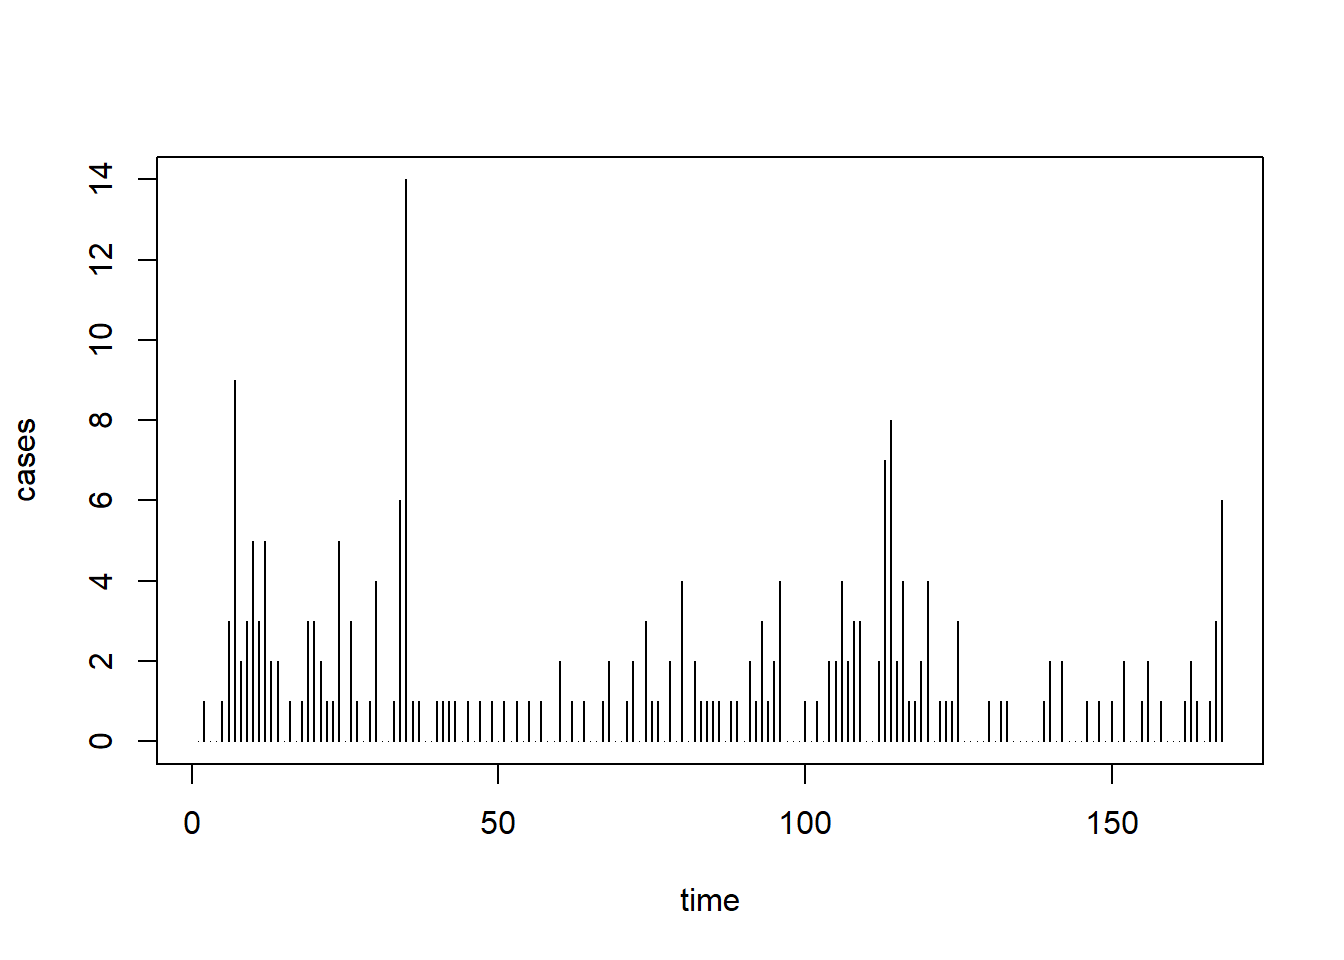
\includegraphics{_main_files/figure-latex/plotpolio2-1.pdf}

Note that the main question we wish to consider is: \emph{How has Polio incidence changed over time?}

Since this is count data, we begin by fitting a Poisson model with a linear time trend.

\begin{Shaded}
\begin{Highlighting}[]
\CommentTok{\# Poisson model with linear time trend}
\NormalTok{polio.glm }\OtherTok{\textless{}{-}} \FunctionTok{glm}\NormalTok{(cases }\SpecialCharTok{\textasciitilde{}}\NormalTok{ time, }\AttributeTok{family=}\FunctionTok{poisson}\NormalTok{(}\AttributeTok{link=}\NormalTok{log), }\AttributeTok{data=}\NormalTok{uspolio)}

\CommentTok{\# Look at the model summary}
\FunctionTok{summary}\NormalTok{(polio.glm)}
\end{Highlighting}
\end{Shaded}

\begin{verbatim}
## 
## Call:
## glm(formula = cases ~ time, family = poisson(link = log), data = uspolio)
## 
## Coefficients:
##              Estimate Std. Error z value Pr(>|z|)    
## (Intercept)  0.626639   0.123641   5.068 4.02e-07 ***
## time        -0.004263   0.001395  -3.055  0.00225 ** 
## ---
## Signif. codes:  0 '***' 0.001 '**' 0.01 '*' 0.05 '.' 0.1 ' ' 1
## 
## (Dispersion parameter for poisson family taken to be 1)
## 
##     Null deviance: 343.00  on 167  degrees of freedom
## Residual deviance: 333.55  on 166  degrees of freedom
## AIC: 594.59
## 
## Number of Fisher Scoring iterations: 5
\end{verbatim}

We can then plot the model as follows.

\begin{Shaded}
\begin{Highlighting}[]
\FunctionTok{plot}\NormalTok{(}\DecValTok{1970} \SpecialCharTok{+}\NormalTok{ ((uspolio}\SpecialCharTok{$}\NormalTok{time }\SpecialCharTok{{-}} \DecValTok{1}\NormalTok{)}\SpecialCharTok{/}\DecValTok{12}\NormalTok{), uspolio}\SpecialCharTok{$}\NormalTok{cases, }\AttributeTok{type=}\StringTok{"h"}\NormalTok{)}
\FunctionTok{lines}\NormalTok{(}\DecValTok{1970} \SpecialCharTok{+}\NormalTok{ ((uspolio}\SpecialCharTok{$}\NormalTok{time }\SpecialCharTok{{-}} \DecValTok{1}\NormalTok{)}\SpecialCharTok{/}\DecValTok{12}\NormalTok{), polio.glm}\SpecialCharTok{$}\NormalTok{fitted)}
\end{Highlighting}
\end{Shaded}

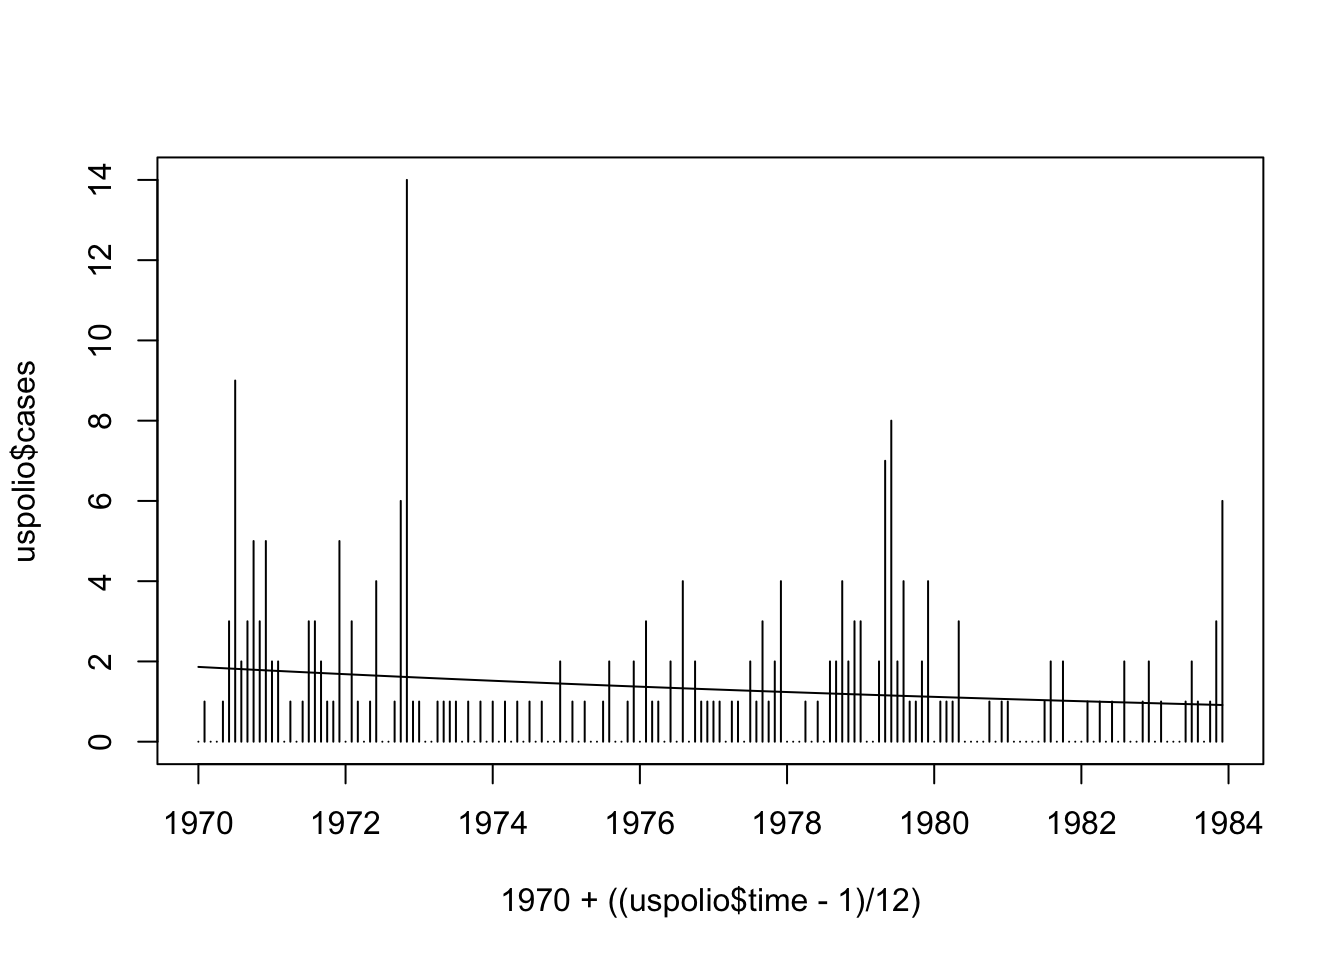
\includegraphics{_main_files/figure-latex/poliopoissonmodelplot-1.pdf}

We can see that this is perhaps unsatisfactory. To improve the model, we can explore a linear trend with seasonal (annual) components.

\begin{Shaded}
\begin{Highlighting}[]
\CommentTok{\# Poisson model with linear trend and annual components}
\NormalTok{polio1.glm }\OtherTok{\textless{}{-}} \FunctionTok{glm}\NormalTok{(cases }\SpecialCharTok{\textasciitilde{}}\NormalTok{ time }\SpecialCharTok{+} \FunctionTok{I}\NormalTok{(}\FunctionTok{cos}\NormalTok{(}\DecValTok{2}\SpecialCharTok{*}\NormalTok{pi}\SpecialCharTok{*}\NormalTok{time}\SpecialCharTok{/}\DecValTok{12}\NormalTok{)) }\SpecialCharTok{+} \FunctionTok{I}\NormalTok{(}\FunctionTok{sin}\NormalTok{(}\DecValTok{2}\SpecialCharTok{*}\NormalTok{pi}\SpecialCharTok{*}\NormalTok{time}\SpecialCharTok{/}\DecValTok{12}\NormalTok{)),}
\AttributeTok{family=}\FunctionTok{poisson}\NormalTok{(}\AttributeTok{link=}\NormalTok{log), }\AttributeTok{data=}\NormalTok{uspolio)}

\FunctionTok{summary}\NormalTok{(polio1.glm)}
\end{Highlighting}
\end{Shaded}

\begin{verbatim}
## 
## Call:
## glm(formula = cases ~ time + I(cos(2 * pi * time/12)) + I(sin(2 * 
##     pi * time/12)), family = poisson(link = log), data = uspolio)
## 
## Coefficients:
##                           Estimate Std. Error z value Pr(>|z|)    
## (Intercept)               0.606612   0.124800   4.861 1.17e-06 ***
## time                     -0.004644   0.001401  -3.315 0.000916 ***
## I(cos(2 * pi * time/12))  0.181254   0.096160   1.885 0.059442 .  
## I(sin(2 * pi * time/12)) -0.423187   0.097590  -4.336 1.45e-05 ***
## ---
## Signif. codes:  0 '***' 0.001 '**' 0.01 '*' 0.05 '.' 0.1 ' ' 1
## 
## (Dispersion parameter for poisson family taken to be 1)
## 
##     Null deviance: 343.00  on 167  degrees of freedom
## Residual deviance: 310.72  on 164  degrees of freedom
## AIC: 575.77
## 
## Number of Fisher Scoring iterations: 5
\end{verbatim}

\begin{Shaded}
\begin{Highlighting}[]
\FunctionTok{plot}\NormalTok{(}\DecValTok{1970} \SpecialCharTok{+}\NormalTok{ ((uspolio}\SpecialCharTok{$}\NormalTok{time }\SpecialCharTok{{-}} \DecValTok{1}\NormalTok{)}\SpecialCharTok{/}\DecValTok{12}\NormalTok{), uspolio}\SpecialCharTok{$}\NormalTok{cases, }\AttributeTok{type=}\StringTok{"h"}\NormalTok{)}
\FunctionTok{lines}\NormalTok{(}\DecValTok{1970} \SpecialCharTok{+}\NormalTok{ ((uspolio}\SpecialCharTok{$}\NormalTok{time }\SpecialCharTok{{-}} \DecValTok{1}\NormalTok{)}\SpecialCharTok{/}\DecValTok{12}\NormalTok{), polio1.glm}\SpecialCharTok{$}\NormalTok{fitted, }\AttributeTok{col=}\DecValTok{2}\NormalTok{)}
\end{Highlighting}
\end{Shaded}

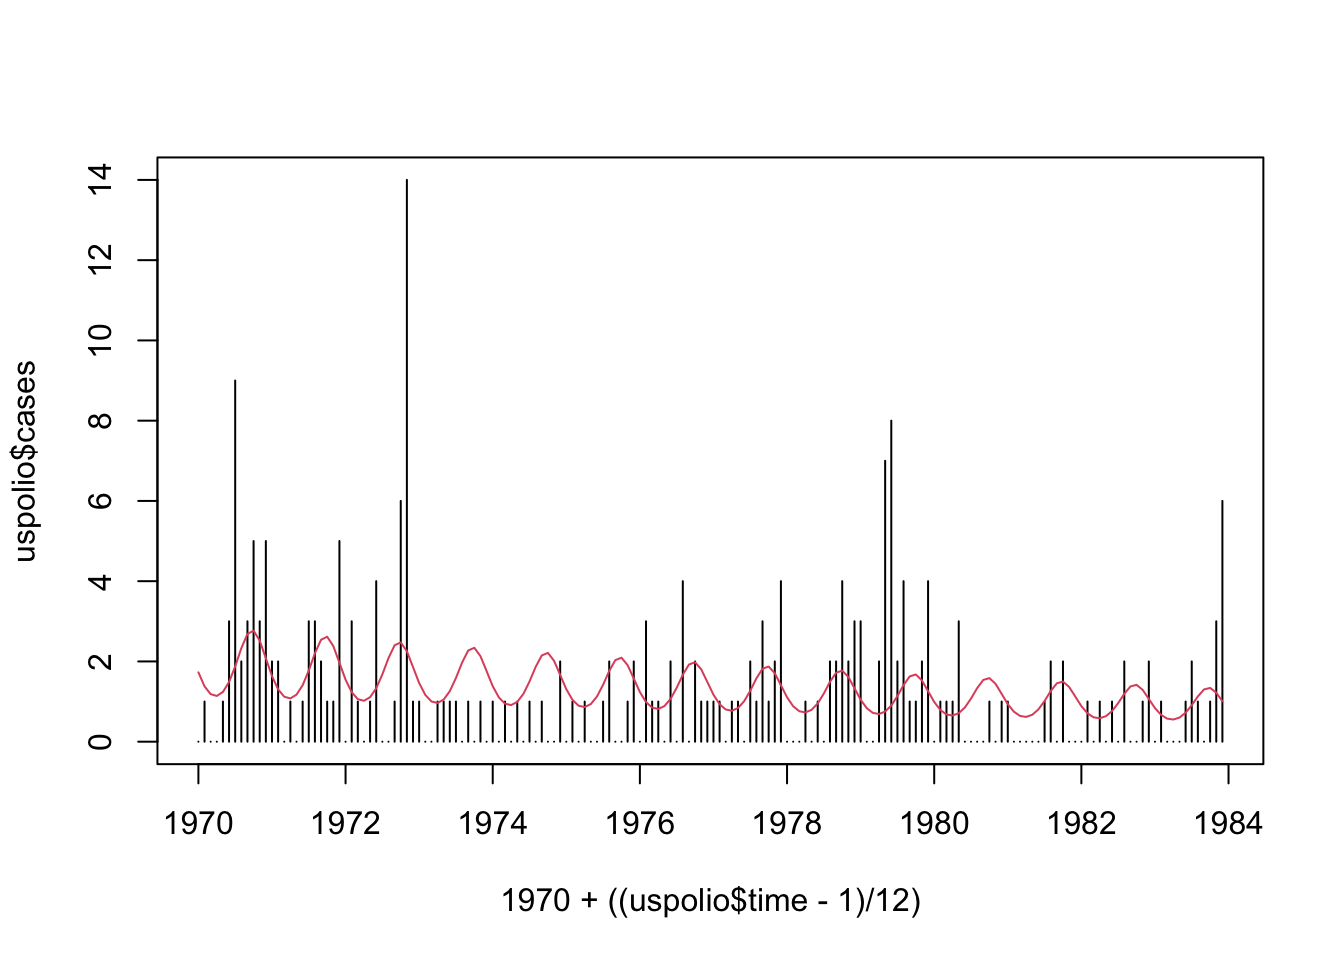
\includegraphics{_main_files/figure-latex/poliopoissonannual-1.pdf}

We can also add six-monthly components into the model.

\begin{Shaded}
\begin{Highlighting}[]
\CommentTok{\# Poisson model with linear trend and seasonal (annual + six{-}monthly) components}
\NormalTok{polio2.glm }\OtherTok{\textless{}{-}} \FunctionTok{glm}\NormalTok{(cases }\SpecialCharTok{\textasciitilde{}}\NormalTok{ time }\SpecialCharTok{+} \FunctionTok{I}\NormalTok{(}\FunctionTok{cos}\NormalTok{(}\DecValTok{2}\SpecialCharTok{*}\NormalTok{pi}\SpecialCharTok{*}\NormalTok{time}\SpecialCharTok{/}\DecValTok{12}\NormalTok{)) }\SpecialCharTok{+} \FunctionTok{I}\NormalTok{(}\FunctionTok{sin}\NormalTok{(}\DecValTok{2}\SpecialCharTok{*}\NormalTok{pi}\SpecialCharTok{*}\NormalTok{time}\SpecialCharTok{/}\DecValTok{12}\NormalTok{))}
\SpecialCharTok{+} \FunctionTok{I}\NormalTok{(}\FunctionTok{cos}\NormalTok{(}\DecValTok{2}\SpecialCharTok{*}\NormalTok{pi}\SpecialCharTok{*}\NormalTok{time}\SpecialCharTok{/}\DecValTok{6}\NormalTok{)) }\SpecialCharTok{+} \FunctionTok{I}\NormalTok{(}\FunctionTok{sin}\NormalTok{(}\DecValTok{2}\SpecialCharTok{*}\NormalTok{pi}\SpecialCharTok{*}\NormalTok{time}\SpecialCharTok{/}\DecValTok{6}\NormalTok{)), }\AttributeTok{family=}\FunctionTok{poisson}\NormalTok{(}\AttributeTok{link=}\NormalTok{log),}
\AttributeTok{data=}\NormalTok{uspolio)}

\FunctionTok{summary}\NormalTok{(polio2.glm)}
\end{Highlighting}
\end{Shaded}

\begin{verbatim}
## 
## Call:
## glm(formula = cases ~ time + I(cos(2 * pi * time/12)) + I(sin(2 * 
##     pi * time/12)) + I(cos(2 * pi * time/6)) + I(sin(2 * pi * 
##     time/6)), family = poisson(link = log), data = uspolio)
## 
## Coefficients:
##                           Estimate Std. Error z value Pr(>|z|)    
## (Intercept)               0.557241   0.127303   4.377 1.20e-05 ***
## time                     -0.004799   0.001403  -3.421 0.000625 ***
## I(cos(2 * pi * time/12))  0.137132   0.089479   1.533 0.125384    
## I(sin(2 * pi * time/12)) -0.534985   0.115476  -4.633 3.61e-06 ***
## I(cos(2 * pi * time/6))   0.458797   0.101467   4.522 6.14e-06 ***
## I(sin(2 * pi * time/6))  -0.069627   0.098123  -0.710 0.477957    
## ---
## Signif. codes:  0 '***' 0.001 '**' 0.01 '*' 0.05 '.' 0.1 ' ' 1
## 
## (Dispersion parameter for poisson family taken to be 1)
## 
##     Null deviance: 343.00  on 167  degrees of freedom
## Residual deviance: 288.85  on 162  degrees of freedom
## AIC: 557.9
## 
## Number of Fisher Scoring iterations: 5
\end{verbatim}

\begin{Shaded}
\begin{Highlighting}[]
\FunctionTok{plot}\NormalTok{(}\DecValTok{1970} \SpecialCharTok{+}\NormalTok{ ((uspolio}\SpecialCharTok{$}\NormalTok{time }\SpecialCharTok{{-}} \DecValTok{1}\NormalTok{)}\SpecialCharTok{/}\DecValTok{12}\NormalTok{), uspolio}\SpecialCharTok{$}\NormalTok{cases, }\AttributeTok{type=}\StringTok{"h"}\NormalTok{)}
\FunctionTok{lines}\NormalTok{(}\DecValTok{1970} \SpecialCharTok{+}\NormalTok{ ((uspolio}\SpecialCharTok{$}\NormalTok{time }\SpecialCharTok{{-}} \DecValTok{1}\NormalTok{)}\SpecialCharTok{/}\DecValTok{12}\NormalTok{), polio2.glm}\SpecialCharTok{$}\NormalTok{fitted, }\AttributeTok{col=}\DecValTok{3}\NormalTok{)}
\end{Highlighting}
\end{Shaded}

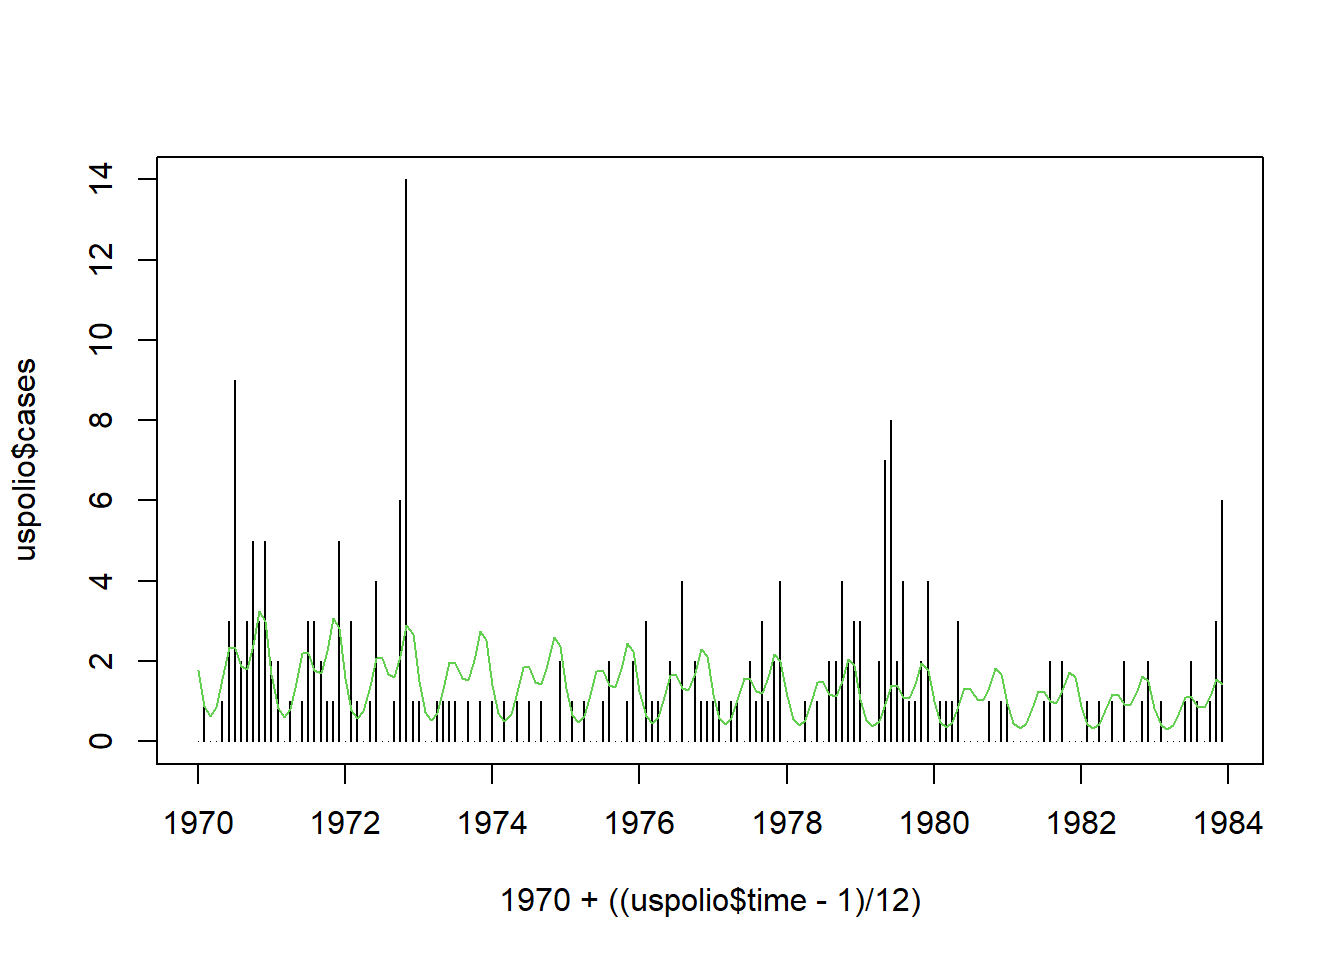
\includegraphics{_main_files/figure-latex/poliopoissonsizmonthly-1.pdf}

Assuming we have annual temperature data over the 14 years, we can add them into the model to investigate their effects.

\begin{Shaded}
\begin{Highlighting}[]
\CommentTok{\# Average annual temperature data over the 14 years}
\NormalTok{temp\_data }\OtherTok{\textless{}{-}} \FunctionTok{rep}\NormalTok{(}\FunctionTok{c}\NormalTok{(}\FloatTok{5.195}\NormalTok{, }\FloatTok{5.138}\NormalTok{, }\FloatTok{5.316}\NormalTok{, }\FloatTok{5.242}\NormalTok{, }\FloatTok{5.094}\NormalTok{, }\FloatTok{5.108}\NormalTok{, }\FloatTok{5.260}\NormalTok{, }\FloatTok{5.153}\NormalTok{, }
                   \FloatTok{5.155}\NormalTok{, }\FloatTok{5.231}\NormalTok{, }\FloatTok{5.234}\NormalTok{, }\FloatTok{5.142}\NormalTok{, }\FloatTok{5.173}\NormalTok{, }\FloatTok{5.167}\NormalTok{), }\AttributeTok{each=}\DecValTok{12}\NormalTok{)}

\CommentTok{\# Scale the data so that it plots nicely}
\NormalTok{scaled\_temp }\OtherTok{=} \DecValTok{10} \SpecialCharTok{*}\NormalTok{ (temp\_data }\SpecialCharTok{{-}} \FunctionTok{min}\NormalTok{(temp\_data))}\SpecialCharTok{/}\NormalTok{(}\FunctionTok{max}\NormalTok{(temp\_data) }\SpecialCharTok{{-}} \FunctionTok{min}\NormalTok{(temp\_data))}
\NormalTok{uspolio}\SpecialCharTok{$}\NormalTok{temp }\OtherTok{=}\NormalTok{ scaled\_temp}

\CommentTok{\# Plot temperature data against cases data to see interest}
\FunctionTok{plot}\NormalTok{(}\DecValTok{1970} \SpecialCharTok{+}\NormalTok{ ((uspolio}\SpecialCharTok{$}\NormalTok{time }\SpecialCharTok{{-}} \DecValTok{1}\NormalTok{)}\SpecialCharTok{/}\DecValTok{12}\NormalTok{), uspolio}\SpecialCharTok{$}\NormalTok{cases, }\AttributeTok{type=}\StringTok{"h"}\NormalTok{)}
\FunctionTok{lines}\NormalTok{(}\DecValTok{1970} \SpecialCharTok{+}\NormalTok{ ((uspolio}\SpecialCharTok{$}\NormalTok{time }\SpecialCharTok{{-}} \DecValTok{1}\NormalTok{)}\SpecialCharTok{/}\DecValTok{12}\NormalTok{), uspolio}\SpecialCharTok{$}\NormalTok{temp, }\AttributeTok{col=}\StringTok{"red"}\NormalTok{)}
\end{Highlighting}
\end{Shaded}

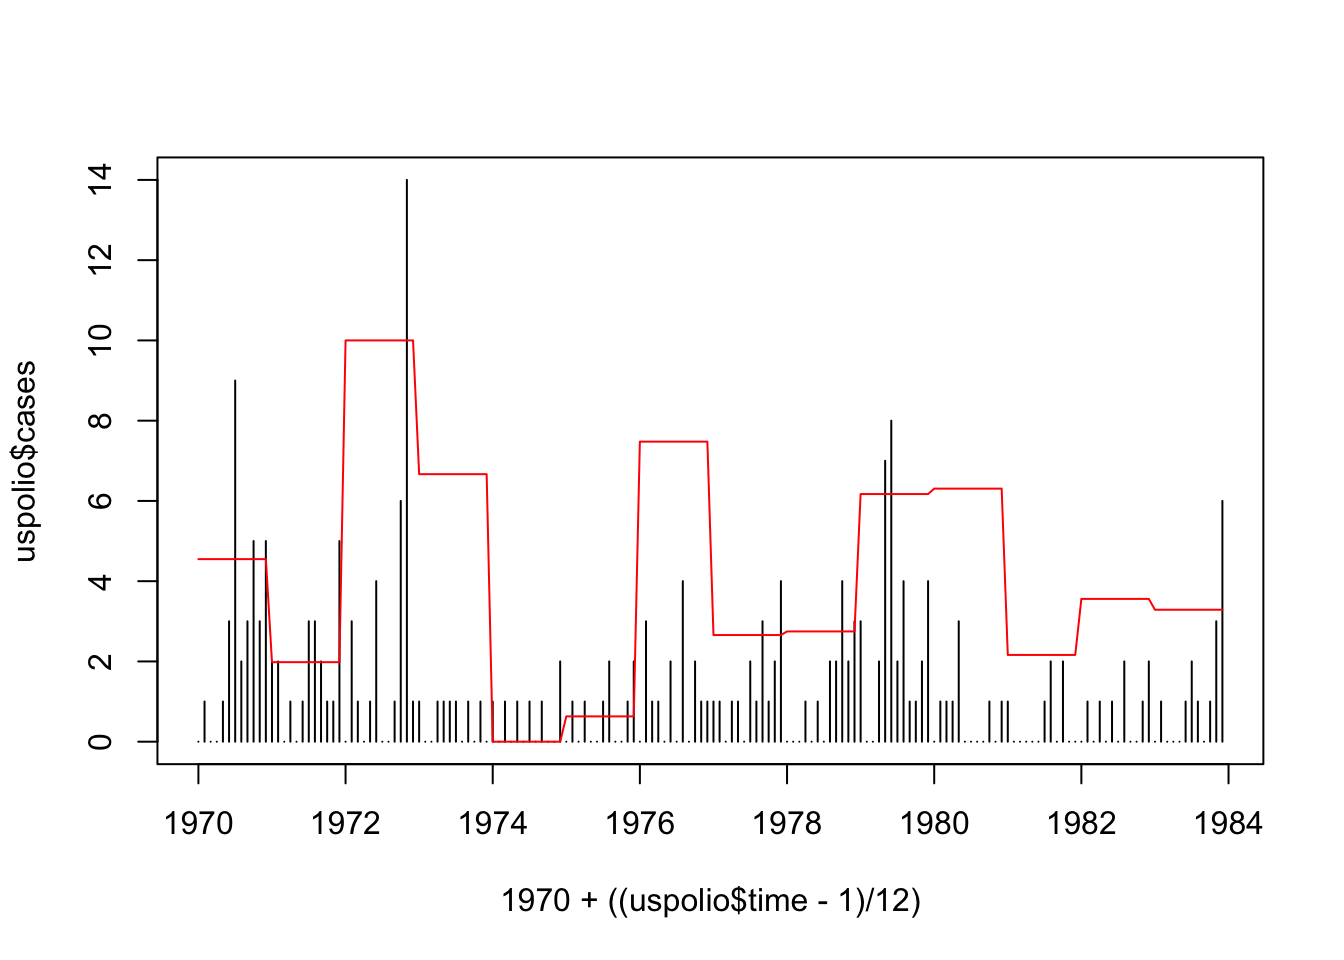
\includegraphics{_main_files/figure-latex/polioaddtempdata-1.pdf}

Poisson GLM with temperature data.

\begin{Shaded}
\begin{Highlighting}[]
\CommentTok{\# Poisson model with additional temperature covariate}
\NormalTok{polio3.glm }\OtherTok{\textless{}{-}} \FunctionTok{glm}\NormalTok{(cases }\SpecialCharTok{\textasciitilde{}}\NormalTok{ time }\SpecialCharTok{+}\NormalTok{ temp }\SpecialCharTok{+} \FunctionTok{I}\NormalTok{(}\FunctionTok{cos}\NormalTok{(}\DecValTok{2}\SpecialCharTok{*}\NormalTok{pi}\SpecialCharTok{*}\NormalTok{time}\SpecialCharTok{/}\DecValTok{12}\NormalTok{)) }\SpecialCharTok{+} \FunctionTok{I}\NormalTok{(}\FunctionTok{sin}\NormalTok{(}\DecValTok{2}\SpecialCharTok{*}\NormalTok{pi}\SpecialCharTok{*}\NormalTok{time}\SpecialCharTok{/}\DecValTok{12}\NormalTok{))}
\SpecialCharTok{+} \FunctionTok{I}\NormalTok{(}\FunctionTok{cos}\NormalTok{(}\DecValTok{2}\SpecialCharTok{*}\NormalTok{pi}\SpecialCharTok{*}\NormalTok{time}\SpecialCharTok{/}\DecValTok{6}\NormalTok{)) }\SpecialCharTok{+} \FunctionTok{I}\NormalTok{(}\FunctionTok{sin}\NormalTok{(}\DecValTok{2}\SpecialCharTok{*}\NormalTok{pi}\SpecialCharTok{*}\NormalTok{time}\SpecialCharTok{/}\DecValTok{6}\NormalTok{)) , }\AttributeTok{family=}\FunctionTok{poisson}\NormalTok{(}\AttributeTok{link=}\NormalTok{log),}
\AttributeTok{data=}\NormalTok{uspolio)}

\FunctionTok{summary}\NormalTok{(polio3.glm)}
\end{Highlighting}
\end{Shaded}

\begin{verbatim}
## 
## Call:
## glm(formula = cases ~ time + temp + I(cos(2 * pi * time/12)) + 
##     I(sin(2 * pi * time/12)) + I(cos(2 * pi * time/6)) + I(sin(2 * 
##     pi * time/6)), family = poisson(link = log), data = uspolio)
## 
## Coefficients:
##                           Estimate Std. Error z value Pr(>|z|)    
## (Intercept)               0.129643   0.186352   0.696 0.486623    
## time                     -0.003972   0.001439  -2.761 0.005770 ** 
## temp                      0.080308   0.023139   3.471 0.000519 ***
## I(cos(2 * pi * time/12))  0.136094   0.089489   1.521 0.128314    
## I(sin(2 * pi * time/12)) -0.531668   0.115466  -4.605 4.13e-06 ***
## I(cos(2 * pi * time/6))   0.457487   0.101435   4.510 6.48e-06 ***
## I(sin(2 * pi * time/6))  -0.068345   0.098149  -0.696 0.486218    
## ---
## Signif. codes:  0 '***' 0.001 '**' 0.01 '*' 0.05 '.' 0.1 ' ' 1
## 
## (Dispersion parameter for poisson family taken to be 1)
## 
##     Null deviance: 343.00  on 167  degrees of freedom
## Residual deviance: 276.84  on 161  degrees of freedom
## AIC: 547.88
## 
## Number of Fisher Scoring iterations: 5
\end{verbatim}

\begin{Shaded}
\begin{Highlighting}[]
\FunctionTok{plot}\NormalTok{(}\DecValTok{1970} \SpecialCharTok{+}\NormalTok{ ((uspolio}\SpecialCharTok{$}\NormalTok{time }\SpecialCharTok{{-}} \DecValTok{1}\NormalTok{)}\SpecialCharTok{/}\DecValTok{12}\NormalTok{), uspolio}\SpecialCharTok{$}\NormalTok{cases, }\AttributeTok{type=}\StringTok{"h"}\NormalTok{)}
\FunctionTok{lines}\NormalTok{(}\DecValTok{1970} \SpecialCharTok{+}\NormalTok{ ((uspolio}\SpecialCharTok{$}\NormalTok{time }\SpecialCharTok{{-}} \DecValTok{1}\NormalTok{)}\SpecialCharTok{/}\DecValTok{12}\NormalTok{), polio3.glm}\SpecialCharTok{$}\NormalTok{fitted, }\AttributeTok{col=}\StringTok{"red"}\NormalTok{)}
\end{Highlighting}
\end{Shaded}

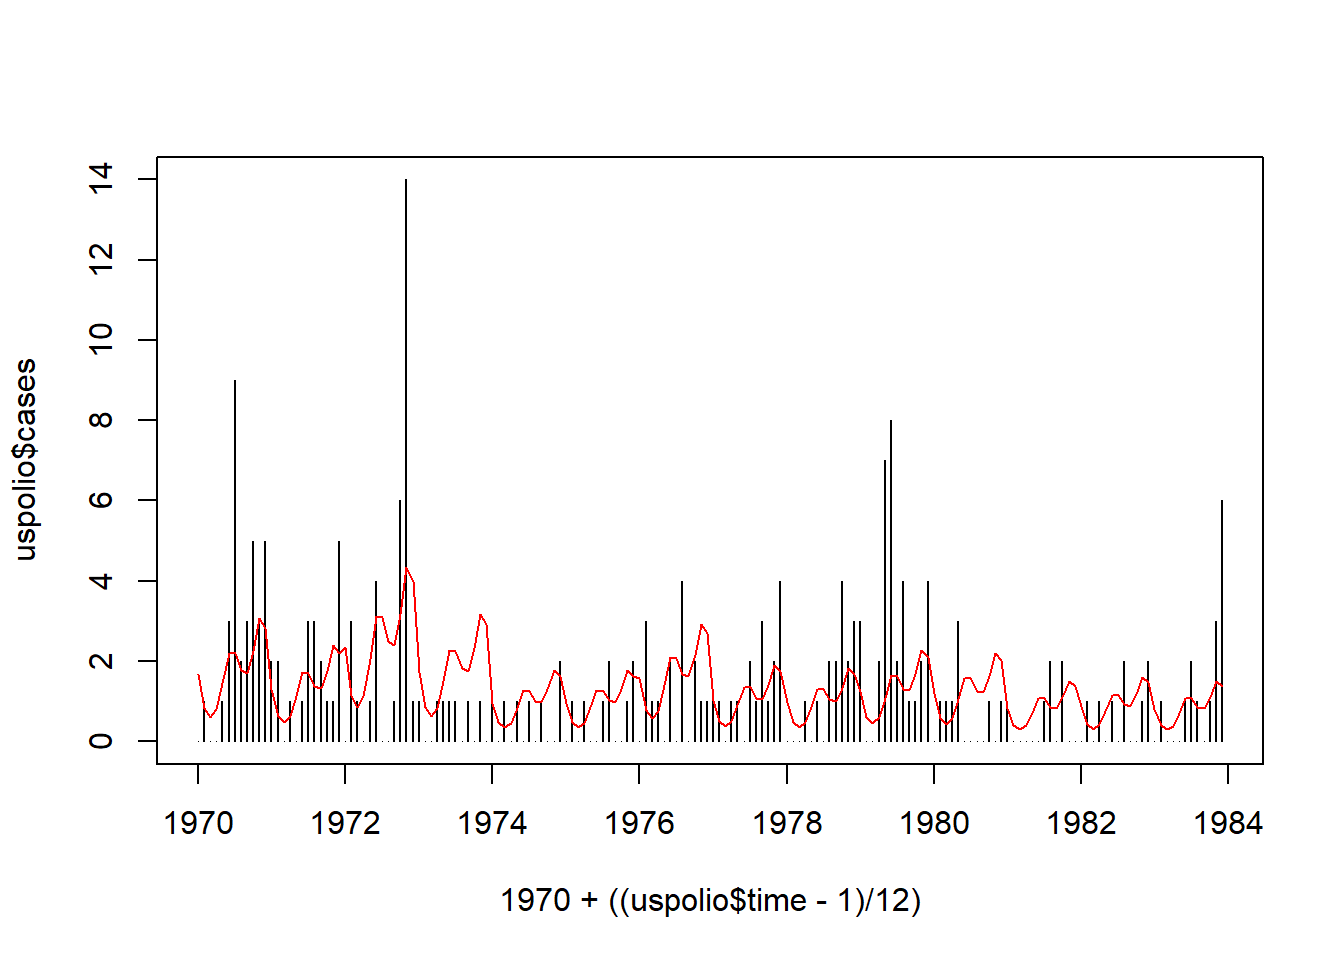
\includegraphics{_main_files/figure-latex/poliopoissontemperature-1.pdf}

\section{\texorpdfstring{Estimation of Dispersion Parameter \(\phi\)}{Estimation of Dispersion Parameter \textbackslash phi}}\label{estimation-of-dispersion-parameter-phi}

Because the dispersion \(\phi\) cancels from the score equation \(\boldsymbol{S}(\hat{\boldsymbol{\beta}}) = 0\), there is no need to estimate \(\phi\) in order to estimate \(\boldsymbol{\beta}\). However, \({\mathrm{Var}}[\hat{\boldsymbol{\beta}}]\) does depend on \(\phi\), as one might expect. Thus, if necessary or of interest, \(\phi\) can be estimated via:

\begin{equation}
  \hat{\phi}
  = \frac{1}{n-p} \sum_{i} m_{i} \frac{(y_{i} - \hat{\mu}_{i})^{2}}{\mathcal{V}(\hat{\mu}_{i})}
  \label{eq:estimatephi}
\end{equation}

where \(p\) is the number of parameters of the model. The motivation for the above estimation is that:

\begin{equation}
  {\mathrm{Var}}[y_{i}]
  = {\mathrm E}[(y_{i} - \mu_{i})^{2}]
  = \phi_{i}\mathcal{V}(\mu_{i})
  = \frac{\phi}{m_{i}} \mathcal{V}(\mu_{i}),
\end{equation}

which can be rearranged to

\begin{equation}
  \phi
  = \frac{m_{i}}{\mathcal{V}(\mu_{i})} {\mathrm E}[(y_{i} - \mu_{i})^{2}]
  = \mathrm{E} \left[ m_{i} \frac{(y_{i} - \mu_{i})^{2}}{\mathcal{V}(\mu_{i})} \right].
\end{equation}

Thus, after estimating \(\hat{\boldsymbol{\beta}}\), we can use its value and Equation \eqref{eq:estimatephi} to estimate \(\hat{\phi}\).

\subsection{Special Cases}\label{special-cases}

\subsubsection{Gaussian}\label{gaussian}

When \(Y |\boldsymbol{\beta}, x \sim {\mathcal N}(\mu, \sigma^{2})\) with \(m_i = 1\), we have \(\mathcal{V}(\mu_{i}) = 1\) and thus,

\begin{equation}
  \hat{\phi} 
  = \frac{1}{n - p} \sum_{i} (y_{i} - \hat{\mu}_{i})^{2}
  = \hat{\sigma}^{2}.
\end{equation}

\subsubsection{Gamma}\label{gamma}

Recall from Exercise 7.1 last term that we can parameterise the Gamma function in terms of its mean \(\mu\) and variance \(\sigma^{2}\), and we found that \(\mathcal{V}(\mu) = \mu^2\). Thus, when \(Y |\boldsymbol{\beta}, x \sim \text{Gamma}(\mu, \sigma^{2})\), we have

\begin{equation}
  \frac{1}{\hat{\nu}}
  = \hat{\phi}
  = \frac{1}{n - p} \sum_{i} m_{i} \frac{(y_{i} - \hat{\mu}_{i})^{2}}{\hat{\mu}_{i}^{2}}.
\end{equation}

\subsection{Practical Example: Hospital Stay Data}\label{practical-example-hospital-stay-data}

In this example, we will use the Hospital Stay data introduced last term to fit a Gamma GLM and estimate its dispersion parameter.

\begin{Shaded}
\begin{Highlighting}[]
\FunctionTok{library}\NormalTok{(npmlreg)}
\FunctionTok{data}\NormalTok{(hosp)}

\CommentTok{\# Fit the GLM and print the summary}
\NormalTok{hosp.glm }\OtherTok{\textless{}{-}} \FunctionTok{glm}\NormalTok{(duration }\SpecialCharTok{\textasciitilde{}}\NormalTok{ age }\SpecialCharTok{+}\NormalTok{ temp1, }\AttributeTok{data=}\NormalTok{hosp, }\AttributeTok{family=}\FunctionTok{Gamma}\NormalTok{(}\AttributeTok{link=}\NormalTok{log))}
\FunctionTok{summary}\NormalTok{(hosp.glm)}
\end{Highlighting}
\end{Shaded}

\begin{verbatim}
## 
## Call:
## glm(formula = duration ~ age + temp1, family = Gamma(link = log), 
##     data = hosp)
## 
## Coefficients:
##               Estimate Std. Error t value Pr(>|t|)  
## (Intercept) -28.654096  16.621018  -1.724   0.0987 .
## age           0.014900   0.005698   2.615   0.0158 *
## temp1         0.306624   0.168141   1.824   0.0818 .
## ---
## Signif. codes:  0 '***' 0.001 '**' 0.01 '*' 0.05 '.' 0.1 ' ' 1
## 
## (Dispersion parameter for Gamma family taken to be 0.2690233)
## 
##     Null deviance: 8.1722  on 24  degrees of freedom
## Residual deviance: 5.7849  on 22  degrees of freedom
## AIC: 142.73
## 
## Number of Fisher Scoring iterations: 6
\end{verbatim}

\begin{Shaded}
\begin{Highlighting}[]
\CommentTok{\# From the summary, note the line:}
\CommentTok{\# (Dispersion parameter for Gamma family taken to be 0.2690233)}

\CommentTok{\# Compute by hand}
\DecValTok{1}\SpecialCharTok{/}\NormalTok{(hosp.glm}\SpecialCharTok{$}\NormalTok{df.res)}\SpecialCharTok{*}\FunctionTok{sum}\NormalTok{((hosp}\SpecialCharTok{$}\NormalTok{duration}\SpecialCharTok{{-}}\NormalTok{hosp.glm}\SpecialCharTok{$}\NormalTok{fitted)}\SpecialCharTok{\^{}}\DecValTok{2}\SpecialCharTok{/}\NormalTok{(hosp.glm}\SpecialCharTok{$}\NormalTok{fitted}\SpecialCharTok{\^{}}\DecValTok{2}\NormalTok{))}
\end{Highlighting}
\end{Shaded}

\begin{verbatim}
## [1] 0.2690233
\end{verbatim}

\section{\texorpdfstring{Asymptotic Properties of \(\hat{\boldsymbol{\beta}}\)}{Asymptotic Properties of \textbackslash hat\{\textbackslash boldsymbol\{\textbackslash beta\}\}}}\label{asymptotic}

In our context, \emph{asymptotic} means that \(M = \sum_{i = 1}^{n} m_{i}\rightarrow \infty\). This could be because \(n\rightarrow \infty\), or because the \(m_{i}\rightarrow\infty\), or a combination of both.

Let us denote the true value of \(\boldsymbol{\beta}\) by \(\boldsymbol{\beta}^*\). In the following, we assume consistency of \(\hat{\boldsymbol{\beta}}\), i.e., \(\hat{\boldsymbol{\beta}}\) converges in probability to \(\boldsymbol{\beta}^*\), meaning that \(P(||\hat{\boldsymbol{\beta}}- \boldsymbol{\beta}^*|| \geq \varepsilon) \rightarrow 0\) as \(n \rightarrow \infty\). We will denote this by \(\hat{\boldsymbol{\beta}}\stackrel{a}{=} \boldsymbol{\beta}^*\). We will also abuse this notation to mean ``tends to asymptotically'' for expectations, i.e., if we write \(E[Z] \stackrel{a}{=} z\), that means \(E[Z] \stackrel{n \rightarrow \infty}{\longrightarrow} z\).

From the consistency assumption, \(\hat{\boldsymbol{\beta}}\) will be close to \(\boldsymbol{\beta}^*\) asymptotically, and we can expand \(\boldsymbol{S}\) around it:

\begin{align}
  \boldsymbol{S}(\hat{\boldsymbol{\beta}}) = 0
  & \stackrel{a}{=} \boldsymbol{S}(\boldsymbol{\beta}^*) +
    \frac{\partial \boldsymbol{S}(\boldsymbol{\beta}^*)}{\partial \boldsymbol{\beta}^{T}}(\hat{\boldsymbol{\beta}}- \boldsymbol{\beta}^*) \\
  & = \boldsymbol{S}(\boldsymbol{\beta}^*)
      -\boldsymbol{F}_{\text{obs}}(\boldsymbol{\beta}^*) (\hat{\boldsymbol{\beta}}- \boldsymbol{\beta}^*)
\end{align}

or equivalently,

\begin{equation}
  \hat{\boldsymbol{\beta}}- \boldsymbol{\beta}^*
  \stackrel{a}{=} \boldsymbol{F}_{\text{obs}}(\boldsymbol{\beta}^*)^{-1} \boldsymbol{S}(\boldsymbol{\beta}^*).
  \label{eq:expandS}
\end{equation}

\subsection{Fisher Scoring}\label{fisher-scoring}

In Section \ref{iterativesolution}, we stated that we often use the (expected) Fisher Information in place of the Observed Fisher Information (known as the Fisher Scoring method). Doing so in the context of asymptotic arguments is acceptable. We can roughly see this as follows. For any \(\boldsymbol{\beta}\),

\begin{equation}
  \frac{1}{n}\boldsymbol{F}_{\text{obs}}(\boldsymbol{\beta})
  = - \frac{1}{n} \frac{\partial l}{\partial \boldsymbol{\beta} \partial \boldsymbol{\beta}^T} (\boldsymbol{\beta}) 
  = - \frac{1}{n} \sum_{i=1}^n \frac{\partial l_i}{\partial \boldsymbol{\beta} \partial \boldsymbol{\beta}^T} (\boldsymbol{\beta})
  \rightarrow - \mathrm{E} \left[\frac{\partial l_1}{\partial \boldsymbol{\beta} \partial \boldsymbol{\beta}^T} (\boldsymbol{\beta}) \right]
  = F_1(\boldsymbol{\beta})
\end{equation}

where \(F_1(\boldsymbol{\beta})\) is the expected Fisher Information for a sample of size \(1\) and we are using the law of large numbers as \(n \rightarrow \infty\) here.
It can be shown (see exercise section) that \(\boldsymbol{F}(\boldsymbol{\beta}) = nF_1(\boldsymbol{\beta})\), thus justifying use of \(\boldsymbol{F}_{\text{obs}}(\boldsymbol{\beta}) \stackrel{a}{=} \boldsymbol{F}(\boldsymbol{\beta})\) in the forthcoming asymptotic arguments.

\subsection{Expectation}\label{expectation}

From Equation \eqref{eq:expandS}, we have:

\begin{equation}
  \hat{\boldsymbol{\beta}}- \boldsymbol{\beta}^*
  \stackrel{a}{=} \boldsymbol{F}_{\text{obs}}(\boldsymbol{\beta}^*)^{-1} \boldsymbol{S}(\boldsymbol{\beta}^*)
  \stackrel{a}{=} \boldsymbol{F}(\boldsymbol{\beta}^*)^{-1} \boldsymbol{S}(\boldsymbol{\beta}^*).
  \label{eq:betaintermsofs}
\end{equation}

Because convergence in probability implies convergence in distribution, this in turn implies that

\begin{equation}
  E[\hat{\boldsymbol{\beta}}- \boldsymbol{\beta}^*]
  \stackrel{a}{=} \boldsymbol{F}(\boldsymbol{\beta}^*)^{-1} E[\boldsymbol{S}(\boldsymbol{\beta}^*)]
  = 0.
\end{equation}

In other words, \(\hat{\boldsymbol{\beta}}\) is asymptotically unbiased.

\subsection{Variance}\label{variance}

Since \(E[\hat{\boldsymbol{\beta}}- \boldsymbol{\beta}^*] \stackrel{a}{=} 0\), we have that

\begin{align}
  {\mathrm{Var}}[\hat{\boldsymbol{\beta}}- \boldsymbol{\beta}^*]
  & \stackrel{a}{=} {\mathrm E}[(\hat{\boldsymbol{\beta}}- \boldsymbol{\beta}^*)(\hat{\boldsymbol{\beta}}- \boldsymbol{\beta}^*)^{T}] \\
  & \stackrel{a}{=} {\mathrm E}[\boldsymbol{F}(\boldsymbol{\beta}^*)^{-1} \boldsymbol{S}(\boldsymbol{\beta}^*)
    \boldsymbol{S}(\boldsymbol{\beta}^*)^{T} \boldsymbol{F}(\boldsymbol{\beta}^*)^{-T}] \\
  & = \boldsymbol{F}(\boldsymbol{\beta}^*)^{-1} {\mathrm E}[\boldsymbol{S}(\boldsymbol{\beta}^*) 
    \boldsymbol{S}(\boldsymbol{\beta}^*)^{T}] \boldsymbol{F}(\boldsymbol{\beta}^*)^{-T} \\
  & = \boldsymbol{F}(\boldsymbol{\beta}^*)^{-1} {\mathrm{Var}}[\boldsymbol{S}(\boldsymbol{\beta}^*)] \boldsymbol{F}(\boldsymbol{\beta}^*)^{-T} \\
  & = \boldsymbol{F}(\boldsymbol{\beta}^*)^{-1}
\end{align}

where we have used symmetry of \(\boldsymbol{F}\) and the fact that \(\boldsymbol{F}(\boldsymbol{\beta}^*) = {\mathrm{Var}}[\boldsymbol{S}(\boldsymbol{\beta}^*)]\).

Thus,

\begin{equation}
  {\mathrm{Var}}[\hat{\boldsymbol{\beta}}] = {\mathrm{Var}}[\hat{\boldsymbol{\beta}}- \boldsymbol{\beta}^*]
  \stackrel{a}{=} \boldsymbol{F}(\boldsymbol{\beta}^*)^{-1}.
  \label{eq:varhbeta}
\end{equation}

\subsection{Asymptotic Normality}\label{asymptotic-normality}

The following is a sketch of the argument of asymptotic normality for \(\hat{\boldsymbol{\beta}}- \boldsymbol{\beta}^*\), i.e., \(\hat{\boldsymbol{\beta}}- \boldsymbol{\beta}^*\) converges asymptotically to a normal distribution. We start from

\begin{equation}
  \boldsymbol{S}(\boldsymbol{\beta}) = \sum_{i} \boldsymbol{S}_{i}(\boldsymbol{\beta})
\end{equation}

where \(\boldsymbol{S}_{i}(\boldsymbol{\beta})\) is defined in Section \ref{properties}. This is a sum of independent random variables with zero mean and finite variance. As the number of terms in the sum tends to infinity, then under a certain condition, the distribution of the sum converges in distribution to a normal distribution. Since \({\mathrm E}[\boldsymbol{S}(\boldsymbol{\beta})] = 0\) and \({\mathrm{Var}}[\boldsymbol{S}(\boldsymbol{\beta})] = \boldsymbol{F}(\boldsymbol{\beta})\), we have:

\begin{equation}
  \boldsymbol{S}(\boldsymbol{\beta}) \stackrel{a}{\sim} {\mathcal N}(0, \boldsymbol{F}(\boldsymbol{\beta})).
\end{equation}

Hence,

\begin{equation}
  \hat{\boldsymbol{\beta}}- \boldsymbol{\beta}^*
  \stackrel{a}{=} \boldsymbol{F}(\boldsymbol{\beta}^*)^{-1} \boldsymbol{S}(\boldsymbol{\beta}^*)
  \stackrel{a}{\sim} {\mathcal N}(0, \boldsymbol{F}(\boldsymbol{\beta}^*)^{-1} \boldsymbol{F}(\boldsymbol{\beta}^*) \boldsymbol{F}(\boldsymbol{\beta}^*)^{-T}).
\end{equation}

Since \(\boldsymbol{F}\) is symmetric and convergence in probability implies convergence in distribution, we have:

\begin{equation}
  \hat{\boldsymbol{\beta}}- \boldsymbol{\beta}^*
  \stackrel{a}{\sim}
  {\mathcal N}(0, \boldsymbol{F}(\boldsymbol{\beta}^*)^{-1}).
  \label{eq:disthbeta}
\end{equation}

This also implies that the square of Mahalanobis distance between \(\hat{\boldsymbol{\beta}}\) and \(\boldsymbol{\beta}^*\) is asymptotically chi-square distributed:

\begin{equation}
  (\hat{\boldsymbol{\beta}}- \boldsymbol{\beta}^*)^{T} \boldsymbol{F}(\boldsymbol{\beta}^*) (\hat{\boldsymbol{\beta}}- \boldsymbol{\beta}^*)
  \stackrel{a}{\sim} \chi^{2}(p)
  \label{eq:distmahalanobishbeta}
\end{equation}

where \(p\) is the number of parameters.

\subsection{Closing The Circle}\label{closing-the-circle}

At the beginning of this section, we assumed that \(\hat{\boldsymbol{\beta}}\) converges in probability to \(\boldsymbol{\beta}^*\). We may want to justify that this assumption is reasonable. Note that under some regularity conditions,

\begin{equation}
  \boldsymbol{F}(\boldsymbol{\beta})^{-1}
  = \left(\sum_{i} m_{i} \ldots \right)^{-1}
  \rightarrow 0
\end{equation}

as \(M\rightarrow\infty\). Thus \(\hat{\boldsymbol{\beta}}\) converges in distribution to a constant random variable, which means that it converges in probability too. This is what we were assuming.

Equations \eqref{eq:varhbeta}, \eqref{eq:disthbeta}, and \eqref{eq:distmahalanobishbeta} remain valid when \(\boldsymbol{F}(\boldsymbol{\beta}^*)\) is replaced by \(\boldsymbol{F}(\hat{\boldsymbol{\beta}})\).

\subsection{Next Step}\label{next-step}

Now that we have seen how to estimate the parameters and some of their sampling properties (asymptotically), we can move on to use these estimates to make inferences: predictions about new values and confidence intervals.

\section{Exercises}\label{exercises-1}

\begin{enumerate}
\def\labelenumi{\arabic{enumi}.}
\item
  Show that \(\boldsymbol{F}(\boldsymbol{\beta}) = nF_1(\boldsymbol{\beta})\), where \(\boldsymbol{F}(\boldsymbol{\beta})\) and \(F_1(\boldsymbol{\beta})\) are the Fisher Information on datasets of size \(n\) and \(1\) respectively.
\item
  Using the notation and argument in Section \ref{asymptotic}, show that \(\boldsymbol{F}(\boldsymbol{\beta}^*) \stackrel{a}{=} \boldsymbol{F}(\hat{\boldsymbol{\beta}})\) and thus we can replace \(\boldsymbol{F}(\boldsymbol{\beta}^*)\) by \(\boldsymbol{F}(\hat{\boldsymbol{\beta}})\) in Equations \eqref{eq:varhbeta}, \eqref{eq:disthbeta}, and \eqref{eq:distmahalanobishbeta}.
\end{enumerate}

  \bibliography{BiblionotesDC.bib}

\end{document}
